\documentclass[a4paper,10pt,twoside]{template/ThesisStyle}
\usepackage{amsmath,amssymb}             % AMS Math
% \usepackage[french]{babel}
\usepackage[latin1]{inputenc}
\usepackage[T1]{fontenc}
\usepackage[left=1.5in,right=1.3in,top=1.1in,bottom=1.1in,includefoot,includehead,headheight=13.6pt]{geometry}
\renewcommand{\baselinestretch}{1.05}

% Table of contents for each chapter

\usepackage[nottoc, notlof, notlot]{tocbibind}
\usepackage{minitoc}
\setcounter{minitocdepth}{2}
\mtcindent=15pt
% Use \minitoc where to put a table of contents

\usepackage{aecompl}

% Glossary / list of abbreviations

\usepackage[intoc]{nomencl}
\renewcommand{\nomname}{List of Abbreviations}

\makenomenclature

% My pdf code

\usepackage{ifpdf}

\ifpdf
  \usepackage[pdftex]{graphicx}
  \DeclareGraphicsExtensions{.jpg}
  \usepackage[a4paper,pagebackref,hyperindex=true]{hyperref}
\else
  \usepackage{graphicx}
  \DeclareGraphicsExtensions{.ps,.eps}
  \usepackage[a4paper,dvipdfm,pagebackref,hyperindex=true]{hyperref}
\fi

\graphicspath{{.}{images/}}

% nicer backref links
\renewcommand*{\backref}[1]{}
\renewcommand*{\backrefalt}[4]{%
\ifcase #1 %
(Not cited.)%
\or
(Cited on page~#2.)%
\else
(Cited on pages~#2.)%
\fi}
\renewcommand*{\backrefsep}{, }
\renewcommand*{\backreftwosep}{ and~}
\renewcommand*{\backreflastsep}{ and~}

% Links in pdf
\usepackage{color}
\definecolor{linkcol}{rgb}{0,0,0.4} 
\definecolor{citecol}{rgb}{0.5,0,0} 

% Change this to change the informations included in the pdf file

% See hyperref documentation for information on those parameters

\hypersetup
{
bookmarksopen=true,
pdftitle="Design and Use of Anatomical Atlases for Radiotherapy",
pdfauthor="Olivier COMMOWICK", 
pdfsubject="Creation of atlases and atlas based segmentation", %subject of the document
%pdftoolbar=false, % toolbar hidden
pdfmenubar=true, %menubar shown
pdfhighlight=/O, %effect of clicking on a link
colorlinks=true, %couleurs sur les liens hypertextes
pdfpagemode=None, %aucun mode de page
pdfpagelayout=SinglePage, %ouverture en simple page
pdffitwindow=true, %pages ouvertes entierement dans toute la fenetre
linkcolor=linkcol, %couleur des liens hypertextes internes
citecolor=citecol, %couleur des liens pour les citations
urlcolor=linkcol %couleur des liens pour les url
}

% definitions.
% -------------------

\setcounter{secnumdepth}{3}
\setcounter{tocdepth}{2}

% Some useful commands and shortcut for maths:  partial derivative and stuff

\newcommand{\pd}[2]{\frac{\partial #1}{\partial #2}}
\def\abs{\operatorname{abs}}
\def\argmax{\operatornamewithlimits{arg\,max}}
\def\argmin{\operatornamewithlimits{arg\,min}}
\def\diag{\operatorname{Diag}}
\newcommand{\eqRef}[1]{(\ref{#1})}

\usepackage{rotating}                    % Sideways of figures & tables
%\usepackage{bibunits}
%\usepackage[sectionbib]{chapterbib}          % Cross-reference package (Natural BiB)
%\usepackage{natbib}                  % Put References at the end of each chapter
                                         % Do not put 'sectionbib' option here.
                                         % Sectionbib option in 'natbib' will do.
\usepackage{fancyhdr}                    % Fancy Header and Footer

% \usepackage{txfonts}                     % Public Times New Roman text & math font
  
%%% Fancy Header %%%%%%%%%%%%%%%%%%%%%%%%%%%%%%%%%%%%%%%%%%%%%%%%%%%%%%%%%%%%%%%%%%
% Fancy Header Style Options

\pagestyle{fancy}                       % Sets fancy header and footer
\fancyfoot{}                            % Delete current footer settings

%\renewcommand{\chaptermark}[1]{         % Lower Case Chapter marker style
%  \markboth{\chaptername\ \thechapter.\ #1}}{}} %

%\renewcommand{\sectionmark}[1]{         % Lower case Section marker style
%  \markright{\thesection.\ #1}}         %

\fancyhead[LE,RO]{\bfseries\thepage}    % Page number (boldface) in left on even
% pages and right on odd pages
\fancyhead[RE]{\bfseries\nouppercase{\leftmark}}      % Chapter in the right on even pages
\fancyhead[LO]{\bfseries\nouppercase{\rightmark}}     % Section in the left on odd pages

\let\headruleORIG\headrule
\renewcommand{\headrule}{\color{black} \headruleORIG}
\renewcommand{\headrulewidth}{1.0pt}
\usepackage{colortbl}
\arrayrulecolor{black}

\fancypagestyle{plain}{
  \fancyhead{}
  \fancyfoot{}
  \renewcommand{\headrulewidth}{0pt}
}

\usepackage{algorithm}
\usepackage[noend]{algorithmic}

%%% Clear Header %%%%%%%%%%%%%%%%%%%%%%%%%%%%%%%%%%%%%%%%%%%%%%%%%%%%%%%%%%%%%%%%%%
% Clear Header Style on the Last Empty Odd pages
\makeatletter

\def\cleardoublepage{\clearpage\if@twoside \ifodd\c@page\else%
  \hbox{}%
  \thispagestyle{empty}%              % Empty header styles
  \newpage%
  \if@twocolumn\hbox{}\newpage\fi\fi\fi}

\makeatother
 
%%%%%%%%%%%%%%%%%%%%%%%%%%%%%%%%%%%%%%%%%%%%%%%%%%%%%%%%%%%%%%%%%%%%%%%%%%%%%%% 
% Prints your review date and 'Draft Version' (From Josullvn, CS, CMU)
\newcommand{\reviewtimetoday}[2]{\special{!userdict begin
    /bop-hook{gsave 20 710 translate 45 rotate 0.8 setgray
      /Times-Roman findfont 12 scalefont setfont 0 0   moveto (#1) show
      0 -12 moveto (#2) show grestore}def end}}
% You can turn on or off this option.
% \reviewtimetoday{\today}{Draft Version}
%%%%%%%%%%%%%%%%%%%%%%%%%%%%%%%%%%%%%%%%%%%%%%%%%%%%%%%%%%%%%%%%%%%%%%%%%%%%%%% 

\newenvironment{maxime}[1]
{
\vspace*{0cm}
\hfill
\begin{minipage}{0.5\textwidth}%
%\rule[0.5ex]{\textwidth}{0.1mm}\\%
\hrulefill $\:$ {\bf #1}\\
%\vspace*{-0.25cm}
\it 
}%
{%

\hrulefill
\vspace*{0.5cm}%
\end{minipage}
}

\let\minitocORIG\minitoc
\renewcommand{\minitoc}{\minitocORIG \vspace{1.5em}}

\usepackage{multirow}
\usepackage{slashbox}

\newenvironment{bulletList}%
{ \begin{list}%
	{$\bullet$}%
	{\setlength{\labelwidth}{25pt}%
	 \setlength{\leftmargin}{30pt}%
	 \setlength{\itemsep}{\parsep}}}%
{ \end{list} }

\newtheorem{definition}{D�finition}
\renewcommand{\epsilon}{\varepsilon}

% centered page environment

\newenvironment{vcenterpage}
{\newpage\vspace*{\fill}\thispagestyle{empty}\renewcommand{\headrulewidth}{0pt}}
{\vspace*{\fill}}





\begin{document}


	\begin{titlepage}

\begin{center}

\noindent{\textbf{\Huge{ERBPI\ \ DOC}}} \\

\vspace*{1.3cm}

\noindent{\textbf{\Large{Easy Robot Behaviour Programming Interface}}} \\
\vspace*{0.3cm}
\noindent{\textbf{\Large{Documentaci\'on}}} \\

\vspace*{2.3cm}

\noindent{\Large{Desarrollo de una interfaz}} \\
\vspace*{0.1cm}
\noindent{\Large{de programaci\'on para talleres}} \\
\vspace*{0.1cm}
\noindent{\Large{de Rob\'otica Educativa}} \\
\vspace*{2.3cm}

\noindent{\large{Departamento de Computaci\'on}} \\
\vspace*{0.1cm}
\noindent{\large{Facultad de Ciencias Exactas y Naturales}} \\
\vspace*{0.1cm}
\noindent{\large{Universidad de Buenos Aires.}} \\
\vspace*{0.1cm}
\noindent{\large{Buenos Aires, Argentina.}} \\

\vspace*{3.1cm}

\end{center}







\begin{center}
\noindent \large 
\begin{tabular}{rl}
	Javier Caccavelli & \url{jcaccav@dc.uba.ar} \\
	Sol Pedre & \url{spedre@dc.uba.ar} \\
	Pablo de Crist\'oforis & \url{pdecris@dc.uba.ar} \\
	Andrea Katz & \url{akatz@dc.uba.ar} \\
	Diego Bendersky & \url{dbenders@dc.uba.ar} \\
\end{tabular}

\end{center}

\end{titlepage}
\sloppy
\titlepage


	\dominitoc

	\pagenumbering{roman}

	\cleardoublepage

	\section*{Agradecimientos}
A QUIEN LE AGRADECEMOS??


	\tableofcontents


	\mainmatter
	%\chapter{Introduction}
\label{chap:intro}
%\minitoc

\section{Illustration Example}

\subsection{A subsection just for fun}

Sorry I won't write your PhD here ;) This small text just to mention that this style supports writing with accents such as in french words (th�se, d�finir, ...). Also I put here a simple way to include an image. This is standard latex. For pdflatex compilation, the extension of the images is jpg. For latex compilation, this is ps or eps. The base folder containing images is set in formatAndDefs.tex, as well as the default extensions added to the image names.

\begin{figure}[!htbp]
  \begin{center}
    \includegraphics[width=0.9\textwidth]{Chapitre1/arctic_control}
  \end{center}
  \caption{A nice image...}
  \label{fig:jolieImage}
\end{figure}

\section{An equation}

Just to show argmin and partial derivative commands.

\begin{equation}
  T = \argmin_T E(T,R,F)
\end{equation}

Regularization:

\begin{equation}
  \pd{T}{t} = \Delta T
\end{equation}

\section{An other section}

Showing a great bullet list environment:

\begin{bulletList}
 \item First point
 \item Second point
% \item Here is an abbreviation reference \nomenclature{DTI}{Diffusion Tensor Imaging} DTI
\end{bulletList}


% #############################
\chapter{Introducci\'on}
\label{cap:intro}
%%%%%%%%%%%%%%%%%%%%%%%%%%%%%%%%%%%%%%%%%%%%%%%%%%%%%%%%%%%%
%% INTRODUCCION
%%%%%%%%%%%%%%%%%%%%%%%%%%%%%%%%%%%%%%%%%%%%%%%%%%%%%%%%%%%%

Realizamos un survey de interfaces gr�ficas de programaci�n.

Estos son todos proyectos para ni�os, la mayor�a implementados para la OLPC (One Laptop Per Child Project):
\begin{itemize}
  \item StarLogo TNG \\ \url{http://education.mit.edu/drupal/starlogo-tng}
  \item EToys (Smalltalk/Squeak) \\ \url{http://wiki.laptop.org/go/Etoys} \\ \url{http://www.squeakland.org/download/}
  \item Scratch (Squeak) \\ \url{http://scratch.mit.edu/}
\end{itemize}

Tambi�n hay un framework de Microsoft:
\begin{itemize}
  \item Microsoft Robotics Developer Studio (RDS)\\ \url{http://msdn.microsoft.com/en-us/library/cc998476.aspx}
	\item Microsoft Visual Programming Language (VPL) \\ \url{http://msdn.microsoft.com/en-us/library/bb483088.aspx}
	\item Microsoft Visual Simulation Environment (VSE) \\ \url{http://msdn.microsoft.com/en-us/library/bb483076.aspx}
\end{itemize}

ARREGLAR ESTO, COMPLETAR CON LO DEL EUROBOT2011 QUE EST\'A MUY BIEN...

% #############################
\chapter{ERBPI: Easy Robot Behaviour Programming Interface}
\label{cap:erbpi}
%%%%%%%%%%%%%%%%%%%%%%%%%%%%%%%%%%%%%%%%%%%%%%%%%%%%%%%%%%%%
%% ERBPI
%%%%%%%%%%%%%%%%%%%%%%%%%%%%%%%%%%%%%%%%%%%%%%%%%%%%%%%%%%%%


La idea general del software es que permita, a trav�s de una interfaz gr�fica y sencilla,
programar los robots para realizar distintas experiencias de veh�culos de Braitenberg y 
comportamiento basado en subsumisi�n\footnote{\textit{Subsumption Architecture}, Behavior-Based Robotics, R. C. Arkin.}.

Para eso, nos basamos en el survey que realizamos, principalmente los programas \textit{StarLogo} y \textit{Scratch}, 
que resultaron los mejorcitos en cuanto a la interfaz gr�fica de programaci�n y la idea de la interfaz gr�fica de proveer menus y submen�es con los objetos predefinidos para ir agregando...

La idea es poder combinar \textit{Braitenberg} y \textit{Subsumisi�n}, de manera que cada estado de la maquina de estados de subsimisi�n sea un braitenberg.
Entonces, en principio, se puede hacer s�lo Braitenberg. Luego, se puede hacer Subsumisi�n ``insertando'' en cada estado un braitenberg 
definido anteriormente.

Algo as� como la Figura \ref{Fig:subsumision}:

\begin{figure}
	\centering
	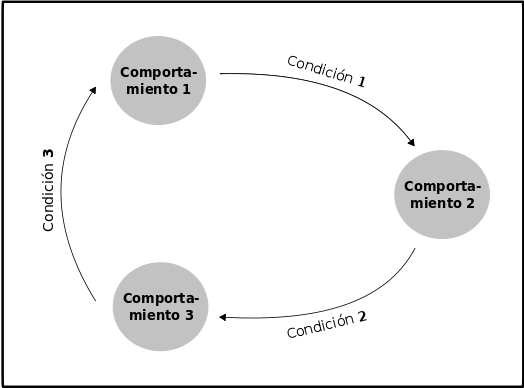
\includegraphics[scale=0.7]{images/subsumision.png}
	\caption{FORMA GENERAL DISE\~nO SOFTWARE.}
	\label{Fig:subsumision}
\end{figure}

ARREGLAR ESTO, COMPLETAR CON LO DEL EUROBOT2011 QUE EST\'A MUY BIEN...

% #############################
\chapter{Dise\~no}
\label{cap:disenio}
%%%%%%%%%%%%%%%%%%%%%%%%%%%%%%%%%%%%%%%%%%%%%%%%%%%%%%%%%%%%
%% DISE�O
%%%%%%%%%%%%%%%%%%%%%%%%%%%%%%%%%%%%%%%%%%%%%%%%%%%%%%%%%%%%


El software estar�a compuesto por tres m�dulos independientes. Un m�dulo \textit{Core}, un m�dulo \textit{RAL} y un m�dulo \textit{GUI}.
Esto nos permite realizar el desarrollo de cada m�dulo completamente por separado.



Algo as� como la Figura \ref{Fig:arq}:

\begin{figure}
	\centering
	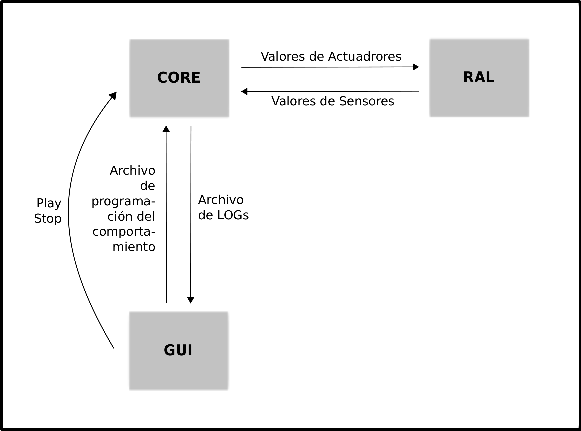
\includegraphics[scale=0.7]{images/arquitectura.png}
	\caption{ERBPI ARQUITECTURA.}
	\label{Fig:arq}
\end{figure}


ARREGLAR ESTO, COMPLETAR CON LO DEL EUROBOT2011 QUE EST\'A MUY BIEN...

% #############################
\chapter{Core}
\label{cap:core}
%%%%%%%%%%%%%%%%%%%%%%%%%%%%%%%%%%%%%%%%%%%%%%%%%%%%%%%%%%%%
%% CORE
%%%%%%%%%%%%%%%%%%%%%%%%%%%%%%%%%%%%%%%%%%%%%%%%%%%%%%%%%%%%



\section{Introducci\'on}

The CORE module is in charge of executing the behaviour. It reads the XML
behaviour file and establishes a connection with the appropriate RAL. At regular
intervals, the core receives from the RAL the normalized values of the sensors,
executes the behaviour, and gives to the RAL the normalized values to set the
actuators. The CORE stops when the GUI signals the user has stopped the
execution.
To be able to execute the behaviour, the CORE has to transform the execu-
tion graph defined by the GUI in the behaviour-file to a corresponding ordered
execution list, to guarantee that all the inputs for a function are ready when its
turn to execute is up. For this, we used a topological sorting [13] of the execution graph. 

The CORE also performs different checkups to assure that the behaviour
can be executed in the selected robot, for example that the graph is not cyclic
(i.e, cannot be ordered) or that the robot has enough sensors and actuators
to execute the behaviour. It also defines the communication frequency with the
RAL depending on the robot, since each robot has a different working frequency.
Finally, the CORE makes a log-file where all the values at a certain time are
registered, including each sensor value, the output value of each function and
the value of each actuator. This log file is communicated to the GUI. We plan
to use it to implement a debug function in the future.

El Core deber�a, a grandes rasgos, hacer las siguientes cosas:

\begin{enumerate}
  \item \textbf{Parsear el XML:} Levantar el archivo XML, chequear que no haya elementos repetidos por \textit{id},
		chequear que no existan ciclos en el grafo formado por los sensores + cajas + actuadores, chequear
		que los predecesores de cada elemento sean elementos existentes de modo que el grafo sea consistente,
		realizar un \textit{topological sorting}\footnote{\textit{Topological Sort, Introduction to Algorithms}, Cormen, Leiserson, Rivest, and Stein.}
		del grafo, y por �ltimo, devolver la \textit{tabla de orden de ejecuci�n secuencial}
		con la cual se realizar� toda la ejecuci�n posterior.
  \item \textbf{Chequear que los sensores y actuadores del Core y el RAL se correpondan entre s�:}
		Obtener la lista de sensores y actuadores del \textit{RAL} y realizar el chequeo de que el \textit{RAL} contenga
		los sensores y actuadores que tiene el \textit{Core}.
  \item \textbf{Definir la frecuencia de trabajo:} Obtener la \textit{frecuencia de trabajo} del \textit{RAL}
		para luego ejecutar como m�ximo a esta \textit{frecuencia}.
  \item \textbf{Ejecutar:} Obtener el nuevo estado (valor) de los sensores del \textit{RAL} y actualizar sus
		valores en la\textit{ tabla de orden de ejecuci�n}, para cada elemento de la \textit{tabla de orden de ejecuci�n}
		actualizar sus valores en funci�n de sus predecesores, y por �ltimo, enviarle al \textit{RAL} el nuevo
		valor para los actuadores y actualizar el archivo de \textit{LOG} con el valor de todos los elementos de
		la tabla de orden de ejecuci�n.
\end{enumerate}

\textbf{Observaciones:}
\begin{itemize}
  \item En el parseo, no se chequea que una \textit{Caja} no tenga como entrada a un \textit{Actuador}.
  \item En el \textit{LOG}, no se guarda el estado de sensores del \textit{RAL}, se desprenden de la \textit{tabla de orden de ejecuci�n}.
  \item En el chequeo entre sensores y actuadores del \textit{Core} y el \textit{RAL},
		no se chequea que est�n en el mismo orden, s�lo que los sensores y actuadores del \textit{Core} sean un subconjunto de
		los sensores y actuadores del \textit{RAL}
\end{itemize}


\section{Implementaci\'on}

Lo hacemos en \texttt{C++} para que sea lo m�s r�pido y potente posible.

Para la funcionalidad de parseo del XML utilizamos el \textit{Xerces XML Parser 3.0.1}\footnote{\textit{Xerces XML Parser 3.0.1}, \url{http://xerces.apache.org/xerces-c/}}
para \texttt{C++}. Recompilamos las librer�as del Xerces de forma est�tica para
que est�n incluidas en el ejecutable del \textit{Core} y no sea necesario transportalas.

El parseo del XML es bastante estricto y flexible al mismo tiempo. S�lo se obtienen del XML los datos necesarios
para la ejecuci�n del Core, cualquier otro atributo o especificaci�n son ignorados. De esta forma, el XML podr�a
contener informaci�n adicional, que el Core ignorar�, pero que servir�a para otros m�dulos como la \textit{GUI}.
Para m�s detalle sobre la estructura que el Core obtiene del XML,
ver ``XML - Datos para la Ejecuci�n del Core'' en el punto \ref{subsub:EjecXML} en la p�gina \pageref{subsub:EjecXML}.

\subsection{Estructuras}
Para realizar el manejo en el \textit{Core} de los sensores, cajas y actuadores,
se utilizar�n los siguientes objetos (\texttt{C++ class}):

\footnotesize	% esto hace que el verbatim se vea chiquitito
\begin{verbatim}
    clase Elemento (es una clase abstracta)
        atributos:
            string _id
            int _valor        // es el valor de salida
            int _entrada      // es la sumatoria de todas sus entradas
            int _tipo         // tipo: sensor, caja o actuador

        m�todos:
            string getId()    // devuelve _id
            int setValor(int) // setea _valor y lo devuelve
            int getValor()    // devuelve _valor
            int getEntrada()  // devuelve _entrada
            int ejecutar()    // es virtual, llama a la de la clase hija...

    clase Sensor (hereda de clase Elemento)
        atributos:
            // ninguno
        m�todos:
            int ejecutar()    // devuelve valor de Elmemento::_valor

    clase Caja (hereda de clase Elemento)
        atributos:
            vector<Elemento*> _entradas;
            vector<Punto> _puntos;
        m�todos:
            int ejecutar()    // para cada "i" en _entradas, acumula *(_entradas[i]).getValor(),
                              // realiza resultado = funci�n(acumulador), y luego, setea
                              // el "resultado" en Elemento::_valor, setea el "acumulador"
                              // en Elemento::_entrada y devuelve Elemento::_valor

    clase Actuador (hereda de clase Elemento)
        atributos:
            vector<Elemento*> _entradas;
        m�todos:
            int ejecutar()    // para cada "i" en _entradas, acumula *(_entradas[i]).getValor()
                              // luego setea el acumulador en Elemento::_valor
                              // y devuelve Elmemento::_valor

    struct Punto
      int x;
      int y;

    string es la clase de C++ STL.
    vector es la clase de C++ STL.
\end{verbatim}
\normalsize	% esto termina el verbatim se vea chiquitito

De esta forma, la \textit{tabla de orden de ejecuci�n secuencial} ser� un vector de la clase \texttt{Elemento}:

\footnotesize	% esto hace que el verbatim se vea chiquitito
\begin{verbatim}
    vector<Elemento> TablaEjecucion
\end{verbatim}
\normalsize	% esto termina el verbatim se vea chiquitito

As�, la ejecuci�n s�lo consistir� en recorrer la tabla secuencialmente y, por cada elemento,
realizar el \texttt{ejecutar()} que se encargar� de obtener los valores requeridos en $\mathcal{O}(1)$,
ya que cada elemento contiene \textit{punteros} a los elementos que le son predecesores: \texttt{TablaEjecucion[i].ejecutar()}

\textbf{Observaciones:}
\begin{itemize}
\item El m�todo \texttt{Caja::ejecutar()}, asume que los 2 puntos est�n ordenados,
	  es decir, \texttt{Caja.\_puntos[0].x} $\leqslant$ \texttt{Caja.\_puntos[1].x}.
	  Por lo tanto, calcular el valor de la funci�n se reduce a 3 casos:
	  \begin{itemize}
	  \item $entrada \leqslant x_0 \quad \Longrightarrow \quad resultado = y_0$
	  \item $entrada \geqslant x_1 \quad \Longrightarrow \quad resultado = y_1$ 
	  \item $x_0 < entrada < x_1 \quad \Longrightarrow \quad resultado = \displaystyle \frac{y_0-y_1}{x_0-x_1}\times(entrada - x_0) + y_0$ (ecuacion de la recta)
	  \end{itemize}

\item Por como est�n dise�adas las clases, y posteriormente los algoritmos, obliga a que los atributos
	  \texttt{\_entradas} y \texttt{\_puntos} sean p�blicos. De lo contrario, habr�a que especificarlos como privados
	  y especificar sus m�todos correspondientes. Que sean atributos p�blicos y no tengan sus m�todos correspondientes, hace que cualquier funci�n pueda
	  modificar a su antojo cualquier atributo de la clase, y que, en los algoritmos como el Parser, para crear
	  los elementos haya que agregar las \texttt{\&(Elemento)} en \texttt{\_entradas} y los puntos en \texttt{\_puntos}
	  manualmente...
\end{itemize}


\subsection{Pseudoc\'odigos}
\subsubsection{\textit{Core}}
\begin{algorithmic}
\STATE \underline{\textit{Preprocesamiento:}}
	\STATE vector$<$Elemento$>$ TablaEjecucion $\longleftarrow$ Parsear(ArchivoXML, TablaEjecucion)
	\IF {(ids sensores en TablaEjecucion) $\nsubseteq$ (ids RAL.getListaSensores())}
        \STATE Error: los sensores no se corresponden y Terminar
	\ENDIF
	\IF {(ids actuadores en TablaEjecucion) $\nsubseteq$ (ids RAL.getListaActuadores())}
        \STATE Error: los actuadores no se corresponden y Terminar
	\ENDIF
	\STATE frecuencia $\longleftarrow$ RAL.getFrecuenciaTrabajo()
\STATE \underline{\textit{Ejecuci�n:}}
	\WHILE{frecuencia lo permita}
		\STATE vector$<<$id;valor$>>$ sensoresRAL $\longleftarrow$ RAL.getEstadoSensores()
		\STATE actualizar el nuevo valor de cada sensor en TablaEjecucion con sensoresRAL
		\FOR{cada elemento $i$ de TablaEjecucion}
		  \STATE TablaEjecucion[i].ejecutar()
		\ENDFOR
		\STATE vector$<<$id;valor$>>$ actuadoresRAL $\longleftarrow$ generado con los actuadores de la TablaEjecucion
		\STATE RAL.setEstadoActuadores(actuadoresRAL)
		\STATE LOG $\longleftarrow$ actualizar con TablaEjecucion
	\ENDWHILE
\end{algorithmic}

\subsubsection{\textit{Parsear(in ArchivoXML, inout TablaEjecucion)}}
\begin{algorithmic}
\STATE vector$<<$tipo:char; id:string; entradas:vector$<$string$>$; puntos:vector$<<$int;int$>>>>$ vectorAuxiliar $\longleftarrow$ generado con cada elemento (sensor, caja o actuador) parseado de ArchivoXML
\FOR{cada elemento $i$ en vectorAuxiliar}
	\IF {$\exists j, j \neq i$ $/$ vectorAuxiliar[j].id $=$ vectorAuxiliar[i].id}
        \STATE Error: hay IDs repetidos y Terminar
	\ENDIF
\ENDFOR
\FOR{cada elemento $i$ en vectorAuxiliar}
  \FOR{cada elemento $j$ en vectorAuxiliar[i].entradas}
	\IF {$\nexists k, 0 \leqslant k < \mathit{long(vectorAuxiliar)}$ $/$ vectorAuxiliar[k].id $=$ vectorAuxiliar[i].entradas[j]}
        \STATE Error: hay elementos que tienen ``entradas'' que no existen y Terminar
	\ENDIF
  \ENDFOR
\ENDFOR
\IF {HayCiclos(vectorAuxiliar)}
	\STATE Error: el grafo contiene ciclos y Terminar
\ENDIF
\STATE vectorAuxiliar $\longleftarrow$ TopologicalSorting(vectorAuxiliar)
\STATE vector$<$Elemento$>$ TablaEjecucion $\longleftarrow$ vac�o
\FOR{cada elemento $i$ en vectorAuxiliar}
  \IF {vectorAuxiliar[i].tipo $=$ Sensor}
	\STATE nuevo sensor(vectorAuxiliar[i].id)
	\STATE sensor.setValor(0)
	\STATE agrego el sensor en TablaEjecucion al final
  \ENDIF
  \IF {vectorAuxiliar[i].tipo $=$ Caja}
	\STATE nuevo caja(vectorAuxiliar[i].id)
	\FOR{cada elemento $j$ en vectorAuxiliar[i].puntos}
	  \STATE agrego vectorAuxiliar[i].puntos[j] en caja.\_puntos al final
	\ENDFOR
	\FOR{cada elemento $j$ en vectorAuxiliar[i].entradas}
	  \FOR{cada elemento $k$ en TablaEjecucion $(0 \leqslant k \leqslant i)$}
		\IF {vectorAuxiliar[i].entradas[j] $=$ TablaEjecucion[k].getId()}
		  \STATE agrego \&(TablaEjecucion[k]) en caja.\_entradas al final
		\ENDIF
	  \ENDFOR
	\ENDFOR
	\STATE agrego la caja en TablaEjecucion al final
  \ENDIF
  \IF {vectorAuxiliar[i].tipo $=$ Actuador}
	\STATE nuevo actuador(vectorAuxiliar[i].id)
	\FOR{cada elemento $j$ en vectorAuxiliar[i].entradas}
	  \FOR{cada elemento $k$ en TablaEjecucion $(0 \leqslant k \leqslant i)$}
		\IF {vectorAuxiliar[i].entradas[j] $=$ TablaEjecucion[k].getId()}
		  \STATE agrego \&(TablaEjecucion[k]) en actuador.\_entradas al final
		\ENDIF
	  \ENDFOR
	\ENDFOR
	\STATE agrego el actuador en TablaEjecucion al final
  \ENDIF
\ENDFOR
\RETURN TablaEjecucion
\end{algorithmic}

\textbf{Observaciones:} Por el momento, al generar el \texttt{vectorAuxiliar} se 
chequea que la \textit{caja} tenga definidos exactamente 2 puntos, de lo contrario, termina con \textit{ERROR}.



\section{Ejecuci\'on}

\subsection{Linux 32 bits}
No es necesario ejecutar el Core manualmente, de esto se encarga la GUI.
\subsubsection{Script}
De todas formas, si se quisera probar manualmente su ejecuci\'on, puede utilizarse el script \textit{ERBPI/src/core/core\_ejecutar.sh}, edit\'andolo y  modific\'andolo con los par\'ametros requeridos.

Para ejecutar el \textit{Core} se deber�n especificar 3 par�metros:
\begin{enumerate}
 \item \textbf{ArchivoXML:} El archivo \textit{XML} a parsear.
 \item \textbf{ArchivoLOG:} El archivo de \textit{LOG} donde se guardar� el \textit{log} de la ejecuci�n. 
 \item \textbf{RAL\_ID:} la especificaci�n del \textit{RAL} que se utilizar�.  
\end{enumerate}
Por ejemplo: \texttt{./core ArchivoXML.xml ArchivoLOG.log RAL\_ID}

donde \texttt{RAL\_ID} podr�a ser: \textit{exabot}, \textit{khepera}, \textit{yaks}, etc.

\subsubsection{Ejecuci�n del Core junto con el RAL}
Como ya dijimos, el \textit{Core} se encuentra compilado con una \textit{librer�a din�mica} del \textit{RAL}.
Por lo tanto, es necesario indicarle al \textit{sistema operativo} d�nde buscar la librer�a din�mica \texttt{libRAL.so}
cuando el \textit{Core} llame a funciones de la misma. De lo contrario, la ejecuci�n falla.

La forma de hacer esto en \textit{Linux} es, en la misma consola donde se ejecutar� el \textit{Core}, ejecutar las siguientes dos l�neas para agregar al sistema operativo un \textit{path} para la b�squeda de librer�as:
\begin{verbatim}
         # LD_LIBRARY_PATH=$LD_LIBRARY_PATH:<path>
         # export LD_LIBRARY_PATH
\end{verbatim}
donde \textit{$<$path$>$} debe ser la ruta (absoluta) donde se encuentra la librer�a din�mica \textit{libRAL.so},
por ejemplo:
\begin{verbatim}
         # LD_LIBRARY_PATH=$LD_LIBRARY_PATH:/home/usuario/desktop/soft_src/ral/src
\end{verbatim}

Tambi�n podr�a modificarse el archivo de configuraci�n del usuario \texttt{.profile} para agregar esta ruta de forma permanente.
Para m�s informaci�n sobre el manejo de librer�as din�micas en \textit{Linux}, puede consultarse \url{http://www.chuidiang.com/clinux/herramientas/librerias.php}

\textbf{IMPORTANTE !!:} Por ahora las librer�as del RAL se llaman todas iguales libRAL.so y vamos pisando
con la que corresponde en la carpeta de ejecuci�n del Core... Luego, hay que hacer un ``if'' en el Core,
para que cargue en tiempo de ejecuci�n la librer�a que corresponda (\textit{libRAL-yaks.so} o \textit{libRAL-exabot.so}).
Tambi�n va a ser necesario tocar unas cositas en el RAL para que esto quede bien.

\subsection{Windows 32 bits}
FALTA COMPLETAR ESTO!!!\\FALTA COMPLETAR ESTO!!!\\FALTA COMPLETAR ESTO!!!\\

\section{Finalizaci�n}
\subsection{Linux 32 bits}
Al comenzar a ejecutar el \textit{Core}, el mismo entra en un \textit{ciclo infinito} en el que va ejecutando
y actualizando los valores de todos los elementos.

Para terminar la ejecuci�n del \textit{Core}, el mismo tiene definida un \textit{rutina de atenci�n de se�ales},
en particular, para la se�al \texttt{SIGINT}, que al ser recibida por el \textit{Core} termina su ejecuci�n
de forma ordenada, cerrando correctamente el archivo de \textit{log}.

Las se�ales se encuentran definidas en la librer�a estandar $<signal.h>$.
Puede verse su especificaci�n en \url{http://publications.gbdirect.co.uk/c_book/chapter9/signal_handling.html}.
La se�al \texttt{SIGINT}, es una se�al de atenci�n interactiva, generalmente generada por
la teclas \texttt{Ctrl+C} en la consola de ejecuci�n, pero que tambi�n puede ser enviada por otro programa.

La idea es que sea la \textit{GUI} la que inicia la ejecuci�n del \textit{Core} y la que termine la ejecuci�n
del mismo enviando la se�al \texttt{SIGINT}.

\subsection{Windows 32 bits}
FALTA COMPLETAR ESTO!!!\\FALTA COMPLETAR ESTO!!!\\FALTA COMPLETAR ESTO!!!\\


\section{Compilaci\'on}
\label{CoreCompilacion}

El c�digo fuente del Core cuenta con los siguientes archivos:
\begin{enumerate}
 \item \textbf{core.cpp} C�digo principal para la ejecuci�n del \textit{Core}.
 \item \textbf{Estructuras.h} Encabezados de las clases utilizadas para la ejecuci�n del \textit{Core}.
 \item \textbf{Estructuras.cpp} C�digo de las clases utilizadas para la ejecuci�n del \textit{Core}.
 \item \textbf{Parser.h} Encabezados de las funciones para el parseo del archivo \textit{XML}.
 \item \textbf{Parser.cpp} C�digo de las funciones para el parseo del archivo \textit{XML}.
\end{enumerate}

Adem�s, el c�digo fuente del Core necesita para su compilaci�n los siguientes archivos del \textit{RAL}:
\begin{enumerate}
 \item \textbf{RAL.h} Encabezados de las funciones del \textit{RAL}.
 \item \textbf{libRAL.so} Librer�a din�mica del \textit{RAL}.
\end{enumerate}
Puede verse la especificaci�n para la compilaci�n de estos archivos del \textit{RAL} en el punto \ref{subsub:CompRAL} en la p�gina \pageref{subsub:CompRAL}.

\subsection{Linux 32 bits}

\subsubsection{Makefile}
El c�digo fuente del Core incluye un archivo \textit{Makefile} con las siguientes funciones para facilitar
la compilaci�n, linkeo est�tico con el \textit{Xerces Parser}, linkeo din�mico con el \textit{RAL} y el testeo del Core:
\begin{enumerate}
 \item \textbf{all:} Ejecuta las funciones \textit{compilar\_core} y \textit{enlazar\_ejecutable}.
 \item \textbf{compilar\_core:} Compila los archivos del c�digo fuente del \textit{Core} generando los objetos (\textit{*.o}) necesarios para la creaci�n del ejecutable del Core de la siguiente manera: \\
						\textit{g++ -c Estructuras.cpp -o Estructuras.o} \\
						\textit{g++ -c Parser.cpp -o Parser.o} \\
						\textit{g++ -c core.cpp -o core.o}
 \item \textbf{enlazar\_ejecutable:} Genera el ejecutable del \textit{Core} (\texttt{test\_core}) enlazando con las \textit{librer�as est�ticas} del \textit{Xerces} y con las \textit{librer�as din�micas} del \textit{RAL} de la siguiente manera: \\
						\textit{g++ -o test\_core core.o Estructuras.o Parser.o -lxerces-c -lpthread -L$<$path$>$ -Bdynamic -lRAL} \\
						donde \textit{$<$path$>$} debe ser la ruta (puede ser relativa) donde se encuentra la librer�a din�mica \textit{libRAL.so}, 
						por ejemplo \texttt{-L../../ral/src}
 \item \textbf{clean:} Borra todos los archivos \textit{*.o} y el ejecutable \textit{test\_core}.
 \item \textbf{run:} Ejecuta \textit{test\_core} con los siguientes par�metros: \\
					  \textit{./test\_core xml\_file\_test\_07.xml archivoLOG\_01.log yaks}
\end{enumerate}

\subsubsection{Script}
Para faculitar algunas cuestiones en la compilacion, tambi\'en se incluye un archivo script ``core\_compilar.sh''. El mismo puede ejecutar simplemente con \texttt{./core\_compilar.sh}.

\subsection{Windows 32 bits}
FALTA COMPLETAR ESTO!!!\\FALTA COMPLETAR ESTO!!!\\FALTA COMPLETAR ESTO!!!


\section{Xerces XML Parser}
ver Cap\'itulo \ref{cap:softadd} en p\'agina \pageref{cap:softadd}



\section{Instalaci\'on}
\subsection{Linux 32 bits}
Para la instalaci\'on se ejecuta el script \textit{ERBPI/src/core/core\_instalar.sh}. Es necesario que el Core y las librer\'ias din\'amicas de cada RAL ya se encuentren compiladas con anterioridad. Para compilaci\'on de Core y RAL ver puntos \ref{CoreCompilacion} y \ref{RalCompilacion}.
\subsection{Windows 32 bits}
FALTA COMPLETAR ESTO!!!\\FALTA COMPLETAR ESTO!!!\\FALTA COMPLETAR ESTO!!!\\


\section{Compiladores}
\subsection{C++ Linux 32 bits}
Utilizamos los siguientes compiladores para C++:
\begin{itemize}
 \item gcc: GCC (GNU Compiler Collection) C compiler.
 \item g++: GCC (GNU Compiler Collection) C++ compiler.
\end{itemize}
Ver \url{http://gcc.gnu.org/}

\subsection{C++ Windows 32 bits}
FALTA COMPLETAR ESTO!!!\\FALTA COMPLETAR ESTO!!!\\FALTA COMPLETAR ESTO!!!\\
FALTA COMPLETAR ESTO!!! Para que los comandos como \textit{gcc}, \textit{g++}, \textit{make} (\textit{mingw32-make}) anden en la consola de windows, es necesario modificar la variable de sistema \texttt{PATH} de Windows y agregar la ruta \url{C:/MinGW/bin}.

FALTA COMPLETAR ESTO!!! Ojo con esto, porque aunque simula el GNU-GCC, no necesariamente todas las librer�a incluidas andan, porque algunas son especificas de
Linux, por ejemplo ``sys/socket.h'', que me parece que en Windows hay que cambiarla por ``winsock.h'0'.
HAY QUE VER BIEN ESTO y ANOTAR !!!!

FALTA COMPLETAR ESTO!!! Nota: cualquier cosa, probar tambi�n Cygwin 5.1.6 (GNU + Cygnus + Windows) que contiene de \url{http://www.cygwin.com/}. ojo con esto porque me parece que s� o s� necesita ``cygwin1.dll'' en la PC para que despu�s pueda andar... Probar!!!



% #############################
\chapter{RAL: Robot Abstraction Layer}
\label{cap:ral}
%%%%%%%%%%%%%%%%%%%%%%%%%%%%%%%%%%%%%%%%%%%%%%%%%%%%%%%%%%%%
%% RAL
%%%%%%%%%%%%%%%%%%%%%%%%%%%%%%%%%%%%%%%%%%%%%%%%%%%%%%%%%%%%


\section{Introducci\'on}
The RAL modules encapsulates all the knowledge of the particular robot or
simulator, providing a standard interface to the CORE module, and dealing with
everything necessary to communicate with the actual robot. The RAL abstracts
the particular robot, its communication protocol, and normalizes the values of
the particular sensors and actuators. In this way, all the specific characteristics of
the robot are transparent to the CORE: the RAL provides a standard interface
that allows the CORE to get the list of sensors and actuators in the robot,
the frequency the robot can work in, the normalized sensor values, and set the
normalized values for the actuators.

To add a new robotic platform for ERBPI to work with, a programmer must
only program a particular RAL for the platform implementing the general RAL
interface. All RALs are implemented as dynamic libraries. In this manner, we can
add new RALs without having to recompile the CORE or the GUI. Moreover,
this allows the CORE to load a different RAL on runtime, without having to
restart the application. This makes ERBPI easily extendable to control different
robots.

La idea es que sea una capa de abstraction respecto del hardware espec�fico que hay del otro lado, es decir, qu� tipo de robot, simulador, qu� tipo y cantidad de sensores y actuadores, etc.
Por lo tanto, para el \textit{Core} va a ser transparente, s�lo se comunicar� con el \textit{RAL} para recibir el estado de los sensores
 y enviar el nuevo estado para los actuadores. Luego, ser� el \textit{RAL} el que se comunicar� directamente con el hardware o simulador seg�n corresponda (Khepera, ExaBot, Yaks, etc.).

Deber�a hacer las siguientes cosas:
\begin{itemize}
  \item \textbf{getListaSensores().} Devolver una lista de IDs de los sensores que posee el hardware o simulador que se se est� utilizando.
  \item \textbf{getListaActuadores().} Devolver una lista de IDs de los actuadores que posee el hardware o simulador que se se est� utilizando.
  \item \textbf{getEstadoSensores().} Devolver una lista de $<$id;valor$>$ con el nuevo estado de cada sensor del hardware o simulador que se se est� utilizando.
  \item \textbf{getFrecuenciaTrabajo().} Devolver a qu� frecuencia sensa y es posible asignarle a los actuadores el hardware o simulador que se se est� utilizando, para que el \textit{Core} lo tenga en cuenta y trabaje a esta frecuencia como m�ximo...
  \item \textbf{setEstadoActuadores().} Recibir una lista de $<$id;valor$>$ con el nuevo valor para cada actuador y actualizar los actuadores en el hardware o simulador que se se est� utilizando.
  \item \textbf{inicializarRAL().} Inicializar el hardware o simulador que se se est� utilizando.
  \item \textbf{finalizarRAL().} Finalizar el hardware o simulador que se se est� utilizando.
  \item \textbf{Comunicaci�n con el Hardware.} Realizar la conexi�n por software con el hardware espec�fico o simulador que se utilizar� y enviar los comandos correspondientes para que se mueva...
\end{itemize}

\section{Implementaci\'on}
Lo hacemos en \texttt{C++} como una \textit{librer�a din�mica multiplataforma} (.DLL o .SO)
para interactuar directamente con el \textit{Core}, sin la necesidad de recompilar el \textit{Core} para distintos \textit{RALs}.
Luego, para interactuar con otro robot o simulador, simplemente se le especificar�
por l�nea de comandos al \textit{Core} cu�l ser� el \textit{RAL\_ID} que se utilizar�.

Por lo tanto, la \textit{librer�a di�mica del RAL} ser� una sola, y el mismo \textit{RAL} deber� poder diferenciar sobre qu� hardware deber� trabajar... �ESTO LO HACEMOS CON UN PAR�METRO? �ESTE PAR�METRO DEBER�A IR EN C/U DE LAS FUNCIONES DEL RAL? RESOLVER ESTO...

Por el momento, la idea es tener las siguientes \textit{RALs}:

To the date, we have implemented RALs for the Khepera [14] and Exabot
[15] robots, and for the YAKS (Yet another Khepera Simulator) [16] and the
Player/Stage [17] simulator adapted for the ExaBot.

\subsection{Normalizaci�n de Valores}
El m\'odulo RAL se encarga adem\'as de normalizar los valores de sensores y actuadores. De esta forma, se abstrae para el m\'odulo GUI c\'omo es el manejo e interpretaci\'on de los valores de cada sensor y actuador dependiendo del robot o simulador que se est\'e utilizando.

Para esto, el m\'odulo GUI s\'olo maneja valores relativos de los sensores y actuadores. Es decir, para sensores maneja valores en el rango \verb=[0:100]= que indican el porcentaje del valor del sensor (\verb=[0%:100%]=). Para motores, maneja valores en el rango \verb=[-100:100]= que indican el porcentaje del valor del motor (\verb=[-100%:100%]=). El m\'odulo RAL recibe del m\'odulo GUI estos valores relativos (normalizados), se encarga de desnormalizarlos adecuadamente en funci\'on del robot o simulador que se est\'e utilizando, y enviar los valores desnormalizados al robot. Cuando el m\'odulo RAL recibe valores del robot, se encarga de normalizarlos (relativizarlos) antes de entregar estos valores al m\'odulo GUI.

Para m\'as informaci\'on de la normalizaci\'on espec\'ifica para cada robot y simulador, ver apartados \ref{normKhepera}, \ref{normYaks}, \ref{normExa} y \ref{normExaSim}.

\section{Ejecuci\'on}
la llama din\'amicamente el Core

FALTA COMPLETAR ESTO!!!\\FALTA COMPLETAR ESTO!!!\\FALTA COMPLETAR ESTO!!!\\

\section{Compilaci\'on}
\label{RalCompilacion}

\subsection{Linux 32 bits - Librer�a Din\'amica}\label{subsub:CompRAL}
El c�digo fuente del \textit{RAL} cuenta con los siguientes archivos:
\begin{enumerate}
 \item \textbf{RAL.h} Encabezados de las funciones para la utilizaci�n de la librer�a din�mica del \textit{RAL}.
 \item \textbf{RAL.cpp} C�digo de las funciones de la librer�a din�mica del \textit{RAL}.
\end{enumerate}

\subsubsection{Makefile}
Adem�s, el c�digo fuente incluye un archivo \textit{Makefile} con las siguientes funciones para facilitar
la compilaci�n de la librer�a din�mica del \textit{RAL}:
\begin{enumerate}
 \item \textbf{all:} Compila y enlaza los archivos del c�digo fuente generando la librer�a din�mica \textit{libRAL.so} de la siguiente manera: \\
						\textit{g++ -c RAL.cpp -o RAL.o} \\
						\textit{ld -o libRAL.so RAL.o -shared} � \textit{g++ -shared -Wl -o libRAL.so RAL.o} (dependiendo el caso)
 \item \textbf{clean:} Borra todos los archivos \textit{*.o} y \textit{*.so} del \textit{RAL}.
\end{enumerate}

Para m�s informaci�n sobre la creaci�n, compilaci�n y enlace de librer�as din�micas en \textit{Linux}, puede consultarse \url{http://www.chuidiang.com/clinux/herramientas/librerias.php}

\subsubsection{Error de Compilaci�n en 64 bits}
Si el Linux es de 64 bits, es probable que falle la compilaci�n de \textit{RAL.cpp}. La soluci�n es agregar en la l�nea de compilaci�n el
par�metro ``\texttt{-fPIC}'', de forma que la l�nea antes indicada quede como ``\textit{g++ -c RAL.cpp -o RAL.o -fPIC}''.


\subsection{Windows 32 bits - Librer�a Din\'amica}

FALTA COMPLETAR ESTO!!!\\FALTA COMPLETAR ESTO!!!\\FALTA COMPLETAR ESTO!!!
FALTA COMPLETAR ESTO!!! Ojo con esto, porque aunque simula el GNU-GCC, no necesariamente todas las librer�a incluidas andan, porque algunas son especificas de
Linux, por ejemplo ``sys/socket.h'', que me parece que en Windows hay que cambiarla por ``winsock.h'0'.
HAY QUE VER BIEN ESTO y ANOTAR !!!!

FALTA COMPLETAR ESTO!!! Nota: cualquier cosa, probar tambi�n Cygwin 5.1.6 (GNU + Cygnus + Windows) que contiene de \url{http://www.cygwin.com/}. ojo con esto porque me parece que s� o s� necesita ``cygwin1.dll'' en la PC para que despu�s pueda andar... Probar!!!



\section{Instalaci\'on}
lo hace la instalacion del Core!!!

FALTA COMPLETAR ESTO!!!\\FALTA COMPLETAR ESTO!!!\\FALTA COMPLETAR ESTO!!!\\

\section{Compiladores}
\subsection{C++ Linux 32 bits}
Utilizamos los siguientes compiladores para C++:
\begin{itemize}
 \item gcc: GCC (GNU Compiler Collection) C compiler.
 \item g++: GCC (GNU Compiler Collection) C++ compiler.
\end{itemize}
Ver \url{http://gcc.gnu.org/}

\subsection{C++ Windows 32 bits}
FALTA COMPLETAR ESTO!!!\\FALTA COMPLETAR ESTO!!!\\FALTA COMPLETAR ESTO!!!\\
FALTA COMPLETAR ESTO!!! Para que los comandos como \textit{gcc}, \textit{g++}, \textit{make} (\textit{mingw32-make}) anden en la consola de windows, es necesario modificar la variable de sistema \texttt{PATH} de Windows y agregar la ruta \url{C:/MinGW/bin}.

FALTA COMPLETAR ESTO!!! Ojo con esto, porque aunque simula el GNU-GCC, no necesariamente todas las librer�a incluidas andan, porque algunas son especificas de
Linux, por ejemplo ``sys/socket.h'', que me parece que en Windows hay que cambiarla por ``winsock.h'0'.
HAY QUE VER BIEN ESTO y ANOTAR !!!!

FALTA COMPLETAR ESTO!!! Nota: cualquier cosa, probar tambi�n Cygwin 5.1.6 (GNU + Cygnus + Windows) que contiene de \url{http://www.cygwin.com/}. ojo con esto porque me parece que s� o s� necesita ``cygwin1.dll'' en la PC para que despu�s pueda andar... Probar!!!



\section{RAL Khepera}
\subsection{Khepera}
\textit{Khepera} es un robot m�vil desarrollado por la empresa K-Team. Tiene un cuerpo
circular, de 5,5\textit{cm} de di�metro, y consta de dos ruedas (actuadores) y ocho pares de sensores
infrarojos, que pueden funcionar como sensores de proximidad o de luz direccionales. Estos
robots pueden ser controlados desde una PC a trav�s de una interface serie o de una interface
de radio.

Para m�s informaci�n ver \cite{kheperaDoc}, \cite{kheperaManual}, \cite{kheperaBase} y \cite{kheperaTurret}.


\subsection{Implementaci\'on}

En funci�n de las especificaciones del robot \textit{Khepera} y las caracter�sticas particulares necesarias para
la conexi�n con el mismo, ya sea a trav�s de \textit{Cable Serial} o \textit{Radio Frecuencia}, realizamos dos \textit{RALs} de \textit{Khepera}, una para 
Linux y otra para Windows.

\subsubsection{Normalizaci\'on de Sensores y Actuadores}
\label{normKhepera}

Los valores absolutos (desnormalizados) y normalizados que maneja el Khepera para sensores y actuadores son:

\begin{tabular}{|r|cc|cc|}
\hline
\textbf{componente} & \textbf{valor m\'inimo} & \textbf{normalizado} & \textbf{valor m\'aximo} & \textbf{normalizado} \\
\hline
sensor proximidad & 0 & 0\% & 1023 & 100\% \\
sensor luz        & 0 & 0\% & 512  & 100\% \\
motores           & -20 & -100\% & 20  & 100\% \\
\hline
\end{tabular} 

La funci\'on de normalizaci\'on-desnormalizaci\'on se encuentra implementada en las funciones \verb=normalizarSensores()= y \verb=desNormalizarMotores()=.
Estas funciones simplemente son una conversi\'on lineal (regla de tres simple) entre el valor del sensor o motor y los valores m\'aximos y m\'inimos. Una vez normalizados o desnormalizados los valores, los mismos son saturados a los valores m\'aximos y m\'inimos permitidos para evitar problemas tanto en el robot como en la GUI. Los valores absolutos posibles para los motores son limitados, aunque el robot Khepera admite valores mayores, no se deben superar los indicados en el rango \verb=[-20:20]= para cuidar la mec\'anica del robot. Para m\'as informaci\'on sobre este punto ver \cite{kheperaManual}(p\'agina 25).

FALTA PONER QU\'E QUIERE DECIR EL VALOR EN MILIMETROS DE \verb=[0:1023]= Y \verb=[0:512]= PARA LOS SENSORES !!!!!\\FALTA PONER QU\'E QUIERE DECIR EL VALOR EN MILIMETROS DE \verb=[0:1023]= Y \verb=[0:512]= PARA LOS SENSORES !!!!!\\FALTA PONER QU\'E QUIERE DECIR EL VALOR EN MILIMETROS DE \verb=[0:1023]= Y \verb=[0:512]= PARA LOS SENSORES !!!!!\\

\textbf{Nota:} tener en cuenta al hacer los c\'alculos de normalizaci\'on-desnormalizaci\'on que deben manejarse los datos en valores \texttt{float} para no perder precisi\'on ni entrar en casos en los que devuelva \textit{cero} por truncamiento a \texttt{int}.


\subsection{Conexi�n por Cable}
Primero es importante chequear que el robot est� correctamente configurado para este tipo de conexi�n.
En la secci�n \textit{3.1.3 - Jumpers, reset button and settings} del manual de usuario se detalla los modos de conexi�n. 
La configuraci�n correcta es \texttt{\textbf{MODE 1}}, que implica una conexi�n \textit{serial RS232 a 9600 Baud}.  Ver Figura \ref{Fig:kheperaJumpersMode}.

\subsubsection{Configuraci\'on Serial RS232}
Para saber c\'omo es el protocolo de comunicaci�n serial ver manual Khepera p\'agina 18, punto \textit{6. The serial communication protocol}.

\textbf{Cuidado:} No hay que tener la torreta puesta y tiene que estar bien configurado el modo de RS232, ver Figura \ref{Fig:kheperaJumpersMode}.

La conexion desde la PC-host siempre es por RS232 y configurada a ``\textit{XXXX Baud, 8 bit, 1 start bit, 2 stop bit, no parity}'', lo �nico que puede cambiar son los \textit{XXXX Baud}, que los configuramos a ``\textit{9600 Baud}'', entonces nuestra configuraci�n de \textit{RS232}:
\begin{itemize}
	\item Port /dev/ttyS0 (para linux)
	\item 9600 Baud
	\item 8 Bit
	\item 1 StartBit
	\item 2 StopBit
	\item NONE Parity
	\item RTS/CTS FlowControl
\end{itemize}

\begin{figure}
	\centering
	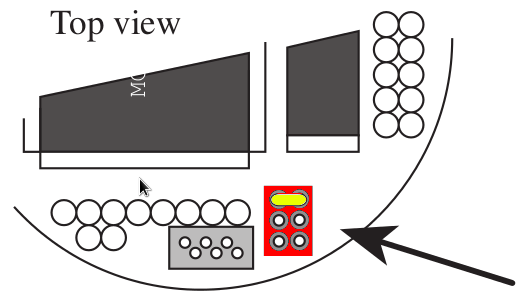
\includegraphics[scale=0.35]{images/khepera_jumpers_mode1b.png}
	\caption{Configuraci\'on de jumpers para el control del robot en ``\textit{Modo 1}'' para el protocolo de comunicaci\'on serial a 9600 Baudios.}
	\label{Fig:kheperaJumpersMode}
\end{figure}

\subsubsection{Alimentaci\'on del robot}
Si el switch de las baterias est� en \textbf{ON:} el robot se power-alimenta de las baterias internas. Si est\'a en \textbf{OFF:} el robot se power-alimenta con el cable serial de datos (6 pines). Ver Figura \ref{Fig:kheperaJumpersBattery}. Ver manual Khepera, p\'agina 15, punto 5.2 \textit{Configuration for robot-computer communication} dice: ``\textit{Between the robot and the interface/charger module by the S serial cable. This cable also supports the power supply of the robot. This external power supply is available when the general battery switch is OFF. If the switch is ON, the robot uses its own batteries for power supply.}''
\begin{figure}
	\centering
	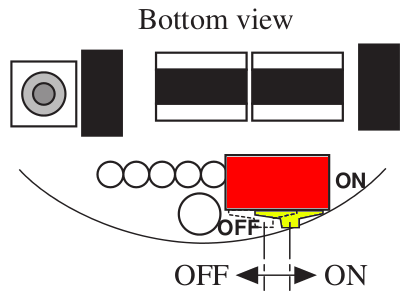
\includegraphics[scale=0.35]{images/khepera_jumpers_batteryb.png}
	\caption{Configuraci\'on de jumpers para el control de la bater\'ia del robot.}
	\label{Fig:kheperaJumpersBattery}
\end{figure}

\subsection{Conexi�n por Radio}
No cambia nada, es lo mismo comunicarse con el robot ``con cable'' y con ``torreta-radio''. Para usar con ``torreta-radio'' s�lo hace falta agregar (enviar) el comando ``\verb=*ID_destination\n='', donde \verb=ID_destination= podr\'ian ser distintos valores en funci\'on de estar utilizando simult\'aneamente distintos robots. En nuestro caso, usamos por defecto el Robot N� 1 por lo que el comando debe ser ``\verb=*1\n='' antes de empezar la transmisi\'on para que el ``radio base'' sepa a qu� robot mandar. Adem\'as, la torreta del khepera en el robot tiene que estar switcheada en ``1'' para aceptar los comandos, o sea, s\'olo trabajaremos con todo configurado en Robot N� 1.
Para simplidicar y unificar las RALs (cable y radio) simplemente agregamos siempre el comando ``\verb=*1\n='', que sirve para \textit{radio} y es ignorado para \textit{cable}.

\subsubsection{Configuraci\'on  Torreta-Radio}
Para usar el robot con \textit{torreta-radio}, adem\'as de montarla sobre el robot, hay que configurar la misma. Ver Figura \ref{Fig:kheperaJumpersTurret}. Ver manual Khepera Radio Turret User, p\'agina 6, punto 4.5 \textit{Running mode and ID selector}. Switches 1 to 6 are used to specify running mode and the radio turret ID. Switches 7 and 8 are not used and have to be always set to 0. Switches 1 to 5 define the 5 bits of the turret ID. Switch 6 defines the running mode of the turret: when this switch is in the OFF position, the turret is a normal extension turret. When this switch is in the ON position, the turret is used as main communication channel of the module COM. We set Switch 1 y 6 to ON, y los switchs 2, 3, 4, 5, 7 y 8 to OFF. The radio turret ID should be never set to 0.

\begin{figure}
	\centering
	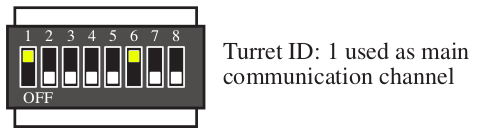
\includegraphics[scale=0.35]{images/khepera_jumpers_turretb.png}
	\caption{Configuraci\'on de jumpers para la torreta-radio del robot.}
	\label{Fig:kheperaJumpersTurret}
\end{figure}


\subsection{RAL Khepera Linux 32 bits}
En Linux, para controlar el puerto serial, o m�s conocido como \texttt{COM1}, se realiza a trav�s del archivo de sistema \url{/dev/ttyS0}, donde en general:
\begin{itemize}
 \item \url{/dev/ttyS0} � \url{/dev/cua0} corresponde con el puerto \texttt{COM1} en Windows
 \item \url{/dev/ttyS1} � \url{/dev/cua1} corresponde con el puerto \texttt{COM2} en Windows
 \item \url{/dev/ttyS2} � \url{/dev/cua2} corresponde con el puerto \texttt{COM3} en Windows
 \item \url{/dev/ttyS3} � \url{/dev/cua3} corresponde con el puerto \texttt{COM4} en Windows
\end{itemize}

Por lo tanto en \texttt{C++}, generar una conexi�n a trav�s del puerto serial, leer, escribir y cerrar el mismo se realiza con las funciones comunes
para manejo de \textit{streams} y archivos:
\footnotesize	% esto hace que el verbatim se vea chiquitito
\begin{verbatim}
        #include <iostream>
        open( "/dev/ttyS0" );
        close( file_descriptor );
        write( file_descriptor );
        read( file_descriptor );
\end{verbatim}
\normalsize	% esto termina el verbatim se vea chiquitito

Es importante el modo en el que se abre el archivo del \texttt{COM1} y m�s importante, configurar el puerto para la conexi�n necesaria para el robot Khepera.
Esto se hace de la sigueinte manera:
\footnotesize	% esto hace que el verbatim se vea chiquitito
\begin{verbatim}
        // se abre el COM1 en modo "non-blocking"
        com1_file_descriptor = open( "/dev/ttyS0", O_RDWR | O_NOCTTY | O_NONBLOCK );
                // O_RDWR - open read-write.
                // O_NOCTTY - open TTY without it becoming controlling tty.
                // O_NONBLOCK � O_NDELAY - open in non-blocking mode (read will return immediately)

\end{verbatim}
\normalsize	% esto termina el verbatim se vea chiquitito

Luego se configura el puerto antes de comenzar a utilizarlo:
\footnotesize	% esto hace que el verbatim se vea chiquitito
\begin{verbatim}
  // se definen constantes para simplificar
  #define BAUDRATE    B9600   // BAUDRATE = 9600
  #define DATABITS_8  CS8     // DATABITS = 8 bits
  #define STOPBITS_2  CSTOPB  // STOPBITS_2 = 2
  #define PARITYON    0       // es igual a PARITY_NONE � PARITY_DISABLED
  #define PARITY      0       // es igual a PARITY_NONE � PARITY_DISABLED
  // se crea la estructura para setear la configuraci�n del puerto
  struct termios com1_new_set;
  com1_new_set.c_cflag = ( BAUDRATE | CRTSCTS | DATABITS_8 | STOPBITS_2 | PARITYON | PARITY | CLOCAL | CREAD );
  com1_new_set.c_iflag = IGNPAR;
  com1_new_set.c_oflag = 0;
  com1_new_set.c_lflag = 0;
  com1_new_set.c_cc[VMIN] = 1;
  com1_new_set.c_cc[VTIME] = 0;
  tcflush( com1_file_descriptor, TCIFLUSH );
  // se setea la nueva configuraci�n para el puerto COM1
  tcsetattr( com1_file_descriptor, TCSANOW, &com1_new_set );
\end{verbatim}
\normalsize	% esto termina el verbatim se vea chiquitito

La compilaci�n de este \textit{RAL} es b�sicamente la misma a la de todos los dem�s, con la diferencia que el proceso
de \textit{linkeo} para generar la librer�a d�namica debi� ser levemente cambiado. El error ocurr�a al intentar \textit{linkear}
el ejecutable del \textit{Core} din�micamente con \textit{libRAL.so}, produc�a el siguiente error:
\footnotesize	% esto hace que el verbatim se vea chiquitito
\begin{verbatim}
   hidden symbol `__dso_handle' in /usr/lib/gcc/i486-linux-gnu/4.3.3/crtbegin.o is referenced by DSO
   /usr/bin/ld: final link failed: Nonrepresentable section on output
   collect2: ld returned 1 exit status
\end{verbatim}
\normalsize	% esto termina el verbatim se vea chiquitito

Por lo tanto, en el \textit{Makefile} inclu�do en los archivos fuentes de este \textit{RAL}, para generar 
la librer�a din�mica \textit{libRAL.so} el proceso de \textit{linkeo} que se realizaba mediante
\textit{ld -o libRAL.so RAL.o -shared} fue cambiado por \textit{\textbf{g++ -shared -Wl -o libRAL.so RAL.o}}.

Por �ltimo, la frecuencia de trabajo que devuelve esta librer�a (\textit{getFrecuenciaTrabajo()}) es igual al
valor que devuelve el \textit{RAL YAKS} (100\textit{mseg}). Seg�n las pruebas que se realizaron parece andar bien, 
pero si aparecieran inconvenientes ser� necesario revisar este valor. Tener en cuenta que la frecuencia de trabajo deber�a
quedar determinada por:
\begin{itemize}
 \item Env�o de comando y tiempo de transmisi�n de esa cantidad de caracteres a 9600 baudios.
 \item Tiempo de sensado (de todos los sensores �16?) del \textit{Khepera}.
 \item Tiempo de transmisi�n de las cantidad de caracteres de la respuesta a 9600 baudios.
 \item Sumatoria de todo lo anterior...
\end{itemize}

Para probar el robot manualmente (chequear que se tiene conexi\'on con el mismo), se pueden instalar y usar los siguientes programas
para el manejo del puerto (como el \textit{hyperterminal} de Windows):
\begin{verbatim}
   sudo apt-get install gtkterm
   sudo apt-get install setserial
\end{verbatim}

\subsubsection{BUGs}
Hay un bug en la ejecuci\'on, ver \ref{bugSA01}

Hay un problema con el RAL Khepera-Torreta-Radio, no anda!!! Ver \ref{bugSA02}



\subsection{RAL Khepera Windows 32 bits}

FALTA COMPLETAR ESTO!!!\\FALTA COMPLETAR ESTO!!!\\FALTA COMPLETAR ESTO!!!\\



\section{RAL YAKS}
\subsection{YAKS}
YAKS es un simulador de c��digo abierto, escrito en \texttt{C++}, de robots tipo \texttt{Khepera}, desarrollado por Johan Carlsson.
Su nombre proviene del acr�nimo \textit{Yet Another Khepera Simulator}. Posee las siguientes caracter�sticas:
\begin{itemize}
 \item Permite incluir en el entorno obst�culos circulares, paredes, luces y definir zonas.
 \item Permite definir y manipular un n�mero ilimitado de robots.
 \item Permite separar el programa de control del simulador, ya que los robots pueden ser manejados a trav�s de una conexi�n \texttt{TCP/IP}.
 \item Soporta una gran variedad de sensores: proximidad, luminosidad, energ�a, encoders de las ruedas, comp�s y sensor de tierra (para detecci�n de zonas).
\end{itemize}

PONER UNA IMAGEN DEL YAKS!!!!!


\subsection{Implementaci\'on}

\subsubsection{Bug}
Hab\'ia un bug en el valor que se seteaba a los motores a diferencia del Khepera. Ver en \ref{bugA04}.

\subsubsection{Normalizaci�n de Sensores y Actuadores}
\label{normYaks}

Los valores absolutos (desnormalizados) y normalizados que maneja el Yaks para sensores y actuadores son:

\begin{tabular}{|r|cc|cc|}
\hline
\textbf{componente} & \textbf{valor m\'inimo} & \textbf{normalizado} & \textbf{valor m\'aximo} & \textbf{normalizado} \\
\hline
sensor proximidad & 0 & 0\% & 1023 & 100\% \\
sensor luz        & 0 & 0\% & 512  & 100\% \\
%motores           & -9 & -100\% & 10  & 100\% \\
motores           & -20 & -100\% & 20  & 100\% \\
\hline
\end{tabular} 

La funci\'on de normalizaci\'on-desnormalizaci\'on se encuentra implementada en las funciones \verb=normalizarSensores()= y \verb=desNormalizarMotores()=.
Estas funciones simplemente son una conversi\'on lineal (regla de tres simple) entre el valor del sensor o motor y los valores m\'aximos y m\'inimos. Una vez normalizados o desnormalizados los valores, los mismos son saturados a los valores m\'aximos y m\'inimos permitidos para evitar problemas tanto en el robot como en la GUI.

Hay que tener mucho cuidado con los valores absolutos que se env\'ian al Yaks para los motores. Por alguna raz\'on de la implementaci\'on del Yaks, si se superan los valores del rango \verb=[-9:10]= el Yaks satura a \texttt{0} (cero) el valor de los motores y el robot no se mueve.
A pesar de esto, por una cuesti\'on de compatibilidad Yaks-Khepera en la GUI, mantuvimos en el Yaks los valores absolutos de motores del Khepera para la desnormalizaci\'on. Luego de esto, saturamos los valores absolutos antes de envi\'arselos al robot dentro del rango \verb=[-9:10]=, esto hace que en el Yaks, los motores nunca superen el rango relativo \verb=[-50%:50%]=.


FALTA PONER QU\'E QUIERE DECIR EL VALOR EN MILIMETROS DE \verb=[0:1023]= Y \verb=[0:512]= PARA LOS SENSORES !!!!!\\FALTA PONER QU\'E QUIERE DECIR EL VALOR EN MILIMETROS DE \verb=[0:1023]= Y \verb=[0:512]= PARA LOS SENSORES !!!!!\\FALTA PONER QU\'E QUIERE DECIR EL VALOR EN MILIMETROS DE \verb=[0:1023]= Y \verb=[0:512]= PARA LOS SENSORES !!!!!\\

\textbf{Nota:} tener en cuenta al hacer los c\'alculos de normalizaci\'on-desnormalizaci\'on que deben manejarse los datos en valores \texttt{float} para no perder precisi\'on ni entrar en casos en los que devuelva \textit{cero} por truncamiento a \texttt{int}.


\section{RAL ExaBot}
\subsection{ExaBot}
\subsection{Implementaci\'on}


\textbf{Nota:} Falta hacer una funci\'on \texttt{inicializarRAL(lista sensores)}, ver bug \ref{bugSA05}.


\subsubsection{Normalizaci�n de Sensores y Actuadores}
\label{normExa}

Los valores absolutos (desnormalizados) y normalizados que maneja el Exabot para sensores y actuadores son:

\begin{tabular}{| p{4.0cm}|p{1,5cm}c|p{1,5cm}c|}
\hline
\textbf{componente} & \textbf{valor m\'inimo} & \textbf{normalizado} & \textbf{valor m\'aximo} & \textbf{normalizado} \\
\hline
sensor infrarrojo de proximidad (tel\'emetro) & 39 & 0\% & 157 & 100\% \\
sensor infrarrojo de l\'inea (line-following) & \verb=[=2:255\verb=]= & 0\% & 1 & 100\% \\
sensor contacto (bumper) & 0 & 0\% & 255 & 100\% \\
sensor radio (sonar) & 31250 & 0\% & 125 & 100\% \\
motores           & -30 & -100\% & 30  & 100\% \\
\hline
\end{tabular} 

La funci\'on de normalizaci\'on-desnormalizaci\'on se encuentra implementada en las funciones \verb=linealizar()=, \verb=normalizarLinea()=, \verb=normalizarBumper()=, \verb=normalizarSonar()= y \verb=setEstadoActuadores()=. A continuaci\'on, y en funci\'on de c\'omo est� configurado el hardware del robot en cada caso, describimos cada una de ellas:

\paragraph{linealizar():}
Esta funci\'on corresponde a la normalizaci\'on de los sensores infrarrojos de proximidad (tel\'emetro). 

Estos sensores arrojan valores entre \verb=[0:159]=. Este rango de valores no se corresponde con una funci\'on lineal, por lo que ser\'a necesario posteriormente linealizar estos valores. De esta forma el primer paso en la normalizaci\'on es traducir el valor absoluto del sensor en un valor de distancia en mil\'imetros, donde $0=800mm$ y $159=60mm$. Notar que al traducir estos valores a distancia, se invierte la relaci\'on de m\'aximo y m\'inimo, ahora el valor \texttt{60mm} es el m\'aximo, donde el tel\'emetro est\'a viendo mucho o un objeto muy cercano, y el valor \texttt{800mm} es el m\'inimo, donde el tel\'emetro est\'a viendo poco o un objeto muy lejano. 

Para linealizar a distancia los valores de estos sensores no se cuenta con una funci\'on. Para esto, se ha desarrollado una tabla de conversi\'on sobre la base de experimentos que indican con qu\'e valores de distancia en mil\'imetros se corresponde cada valor del rango \verb=[0:159]=.

Una vez linealizado el sensor, saturamos los valores. El sensor se encuentra dentro del robot a 70mm del borde del chasis, por lo que a partir de aqu\'i tomaremos nuestra referencia del objeto m\'as cercano, un objecto a 0mm del chasis, es decir, el valor normalizado \texttt{100\%}. Por otro lado, si bien el sensor tiene la capacidad de ver objetos hasta los 800mm, sobre la base de experimentos determinamos m\'as pr\'actico limitar el sensor a los 350mm. Entonces los valores del sensor son saturados en el rango \verb=[39:157]=, que equivale linealmente a \verb=[350mm:70mm]= y relativamente (normalizado) a \verb=[0%:100%]=.

Una vez obtenido linealmente en distancia y saturado el valor del sensor, procedemos a normalizar esta distancia teniendo en cuenta que se encuentran invertidos el m\'aximo y m\'inimo. Para esto simplemente realizamos una conversi\'on lineal (regla de tres simple) entre el valor del sensor y los valores m\'aximos y m\'inimos invertidos. Una vez normalizados estos valores, pueden ser entregados el m\'odulo GUI en el rango \verb=[0%:100%]=.

\paragraph{normalizarLinea():}
Esta funci\'on corresponde a la normalizaci\'on de los sensores infrarrojos de l\'inea (line-following) para detecci\'on de l\'inea blanca en el piso. 

Estos sensores arrojan valores entre \verb=[1:255]= indicando el tiempo transcurrido desde la \'ultima vez que visualiz\'o la l\'inea, donde $255 = \infty \textit{ tiempo}$. En funci\'on de esto, el primer paso ser\'a interpretar estos valores absolutos.

Por una cuesti\'on pr\'actica, en esta funci\'on de normalizaci\'on, interpretaremos el valor absoluto \texttt{1} como que se est\'a viendo la l\'inea en ese preciso momento y los valores absolutos en el rango \verb=[2:255]= como que no se est\'a viendo la l\'inea. 

Como \'ultimo paso, normalizamos los valores absolutos a $1=100\%$ y cualquier otro valor a $0\%$ (valor $\neq 1 \Rightarrow 0\%$)

Tener en cuenta que esta iterpretaci\'on del tiempo devuelto por el sensor podr\'ia cambiarse para obtener linealmente valores de tiempo en milisegundos indicando cu\'ando fue la \'ultima vez que se visualiz\'o la l\'inea.

\paragraph{normalizarBumper():}
Esta funci\'on corresponde a la normalizaci\'on de los sensores de contacto (bumper). 

Estos sensores s\'olo arrojan dos valores \verb=0= y \verb=255=. El valor \verb=0= indica que el sensor est\'a libre (no apretado) y el valor \verb=255= indica que el sensor est\'a apretado. No existe rango de valores.
Por lo que la normalizaci\'on simplemente consiste en que los dos valor absolutos posibles se traducen como $0=0\%$ y $255=100\%$


\paragraph{normalizarSonar():}
Esta funci\'on corresponde a la normalizaci\'on del sensor de radio (sonar). 

Este sensor arroja valores entre \verb=[125:31250]= indicando el tiempo transcurrido desde la \'ultima vez que visualiz\'o un objeto. Estos valores se corresponden con $125 = 100 \mu s = 0.1 ms = 1 cm = 100\%$ y $31250 = 25000 \mu s = 25 ms = 400 cm = 0\%$. Notar que, como en el tel\'emetro, se encuentra invertida la relaci�n de m�ximo y m�nimo, el valor $125 = 1 cm$ es el m�ximo, donde el sonar est� viendo mucho o un objeto muy cercano, y el valor
$31250 = 400 cm$ es el m�nimo, donde el tel�metro est� viendo poco o un objeto muy lejano.

Una vez obtenido e interpretado el valor del sensor, se satura en el rango \verb=[125:31250]= y se procede a normalizar este valor teniendo en cuenta que se encuentran invertidos el m\'aximo y m\'inimo. Para esto simplemente realizamos una conversi\'on lineal (regla de tres simple) entre el valor del sensor y los valores m\'aximos y m\'inimos invertidos. Una vez normalizados estos valores, pueden ser entregados el m\'odulo GUI en el rango \verb=[0%:100%]=.


\paragraph{setEstadoActuadores():}
Esta funci\'on contiene la desnormalizaci\'on (a valores absolutos) de los datos de motores antes de ser enviados al robot. 

La GUI env\'ia a la RAL valores para los motores normalizados en el rango \verb=[-100%:100%]=, por lo que esta funci\'on se encargar\'a de convertir estos valores a valores absolutos para ser entregados al robot en su rango absoluto \verb=[-30:30]=. De esta forma, simplemente se procede a realizar una conversi\'on lineal (regla de tres simple) entre los valores normalizados y desnomalizados, donde $-30 = -100\%$ y $30 = 100\%$. Una vez desnormalizados estos valores, pueden ser entregados al robot en el rango \verb=[-30:30]=.

Una cuesti\'on que se realiza durante el proceso es saturar los valores m\'inimos de los motores. Los motores del ExaBot no funcionan correctamente si se les asigna menos del $20\%$ de su capacidad, por lo que es necesario manejar los valores en estos intervalos peque\~nos. Para esto, definimos la siguiente saturaci\'on de valores antes de desnormalizar:
\begin{center}
\begin{tabular}{ccl}
\verb=(-10:10)= & $\longrightarrow$ & \texttt{0\%} \\
\verb=[10:20)= & $\longrightarrow$ & \texttt{20\%} \\
\verb=(-20:-10]= & $\longrightarrow$ & \texttt{-20\%} \\
\end{tabular} 
\end{center}

Otra cuesti\'on a tener en cuenta es que los motores del robot giran invertidos, por lo que para que ambos motores vayan en el mismo sentido la RAL debe enviar al robot un valor de motor como positivo $(+)$ y otro negativo $(-)$ seg\'un el sentido.

\textbf{Nota:} tener en cuenta al hacer los c\'alculos de normalizaci\'on-desnormalizaci\'on que deben manejarse los datos en valores \texttt{float} para no perder precisi\'on ni entrar en casos en los que devuelva \textit{cero} por truncamiento a \texttt{int}.

\subsection{Conexi�n por UDP}
La conexi\'on con el robot se establece mediante el protocolo UDP. B\'asicamente la implementaci\'on consiste en dos procesos (threads) que corren en paralelo: \verb=udp_receive= y \verb=udp_send=, que comparten la memoria para intercomunicarse mediante un proceso central.

Un detalle importante de la implementaci\'on es que fue necesario configurar como desacoplados del m\'odulo Core a los procesos \verb=udp_receive= y \verb=udp_send=. El Core es el que crea estos procesos y, al terminar el Core, esto tambi\'en terminaba sus procesos hijos (\verb=udp_receive= y \verb=udp_send=) y perd\'iamos la comunicaci\'on con el robot. Para desacoplar (\textit{desatachear}) estos procesos del Core se utiliz\'o la funci\'on \verb=setsid()=.

\subsubsection{Configuraci\'on IP}
Se estableci\'o la siguiente configuraci\'on de direcciones IPs para la conexi\'on UDP:
\footnotesize
\begin{center}
\begin{tabular}{lcccl}
Cable Ethernet IP ExaBot    & $\longrightarrow$ & \verb=0xC0A80032= & $\longrightarrow$ & \verb=192.168.0.50= \\
Cable Ethernet IP PC        & $\longrightarrow$ & \verb=0xC0A80033= & $\longrightarrow$ & \verb=192.168.0.51  | 255.255.255.0 | 192.168.0.1= \\
\\
WiFi IP ExaBot              & $\longrightarrow$ & \verb=0xC0A80132= & $\longrightarrow$ & \verb=192.168.1.50= \\
WiFi IP PC                  & $\longrightarrow$ & \verb=0xC0A801FE= & $\longrightarrow$ & \verb=192.168.1.254 | 255.255.255.0 | 192.168.1.1= \\
\end{tabular} 
\end{center}
\normalsize

\paragraph{Definiciones IPs:}
Las IPs, tanto en el ExaBot como en la RAL-Exabot, est\'an definidas en tiempo de compilaci\'on. Por lo que los ejecutables y librer\'ias din\'amicas tienen definido de antemano la IP (cable o WiFi) a la que se conectar\'an.
Para la RAL, estas definiciones se encuetran en \verb=exabotRAL.h= en las constantes \verb=IP_EXA_CABLE= y \verb=IP_EXA_WIFI=.
Para la aplicaci\'on del robot, estas definiciones se encuetran en \verb=udp_send.c=.

Notar que si las direcciones IPs no coinciden, no s\'olo en los c\'odigos de las aplicaciones que se ejecutan, sino tambi\'en f\'isicamente en las placas de red del robot y la PC host, la conexi\'on no podr\'a ser establecida.

La \textit{submask} y \textit{gateway} no son neesarios, pero conviene definirlos.

\subsection{Software ExaBot para conexi\'on}
El robot cuenta con software espec\'ifico para la conexi\'on UDP, v\'ia cable ethernet y WiFi, para enviar y recibir los comandos necesarios. Para que la GUI pueda comunicarse con el robot, es necesario previamente que la aplicaci\'on de conexi\'on UDP est\'e corriendo en el robot.

\subsubsection{Aplicaci\'on UDP}
La aplicaci�n de conexi�n del robot se encuentra en el ExaBot en su PC embebida en \url{/pc104/1004_codigo_completo}. Se ejecuta desde esa ubicaci\'on con \verb=./test_threads=. Para ampliar los distintos comandos de esta aplicaci\'on ver \ref{????}.

AGREGAR SECCION SOFT ADICIONAL MANUAL DE COMANDOS DEL EXA !!! \\AGREGAR SECCION SOFT ADICIONAL MANUAL DE COMANDOS DEL EXA !!! \\AGREGAR SECCION SOFT ADICIONAL MANUAL DE COMANDOS DEL EXA !!! \\AGREGAR SECCION SOFT ADICIONAL MANUAL DE COMANDOS DEL EXA !!! \\AGREGAR SECCION SOFT ADICIONAL MANUAL DE COMANDOS DEL EXA !!! \\AGREGAR SECCION SOFT ADICIONAL MANUAL DE COMANDOS DEL EXA !!! \\AGREGAR SECCION SOFT ADICIONAL MANUAL DE COMANDOS DEL EXA !!! \\AGREGAR SECCION SOFT ADICIONAL MANUAL DE COMANDOS DEL EXA !!! \\AGREGAR SECCION SOFT ADICIONAL MANUAL DE COMANDOS DEL EXA !!! \\AGREGAR SECCION SOFT ADICIONAL MANUAL DE COMANDOS DEL EXA !!! \\AGREGAR SECCION SOFT ADICIONAL MANUAL DE COMANDOS DEL EXA !!! \\AGREGAR SECCION SOFT ADICIONAL MANUAL DE COMANDOS DEL EXA !!! \\


En esta aplicaci\'on, al igual que en RAL-ExaBot, la IP de conexi\'on a la PC remota (GUI) est\'a definida en tiempo de compilaci\'on, por lo que el ejecutable se encuentra definido de forma fija para un tipo de IP y conexi\'on. Para facilitar esto, ya se encuentran en \url{/usr/bin/} compiladas las dos versiones: \verb=gui_test_threads= (cable ethernet) y \verb=gui_test_threads_254= (WiFi) seg\'un la tabla de IPs anterior.

El ejecutable \verb=gui_test_threads= conectar\'a entre \verb=192.168.0.50= (robot) y \verb=192.168.0.51= (PC host).

El ejecutable \verb=gui_test_threads_254= conectar\'a entre \verb=192.168.1.50= (robot) y \verb=192.168.1.254= (PC host).

Lo m�s c�modo, si es que se utilizar\'a intensivamente el robot junto con la GUI, es que esta aplicaci�n de conexi\'on se ejecute autom�ticamente en el boot del robot.
Para esto, ver \ref{bootExa}

\paragraph{Compilaci\'on:}
Si fuese necesario recompilar esta aplicaci\'on, el c�digo fuente se encuentra en \url{/pc104/1004_codigo_completo} en la PC104. Es necesario conectarse por \verb=telnet 192.168.0.50=, se hace \verb=rm test_threads= y \verb=make test_threads=, y con \verb=./test_threads= se ejecuta para que espere comandos.

\subsubsection{Boot autom\'atico en ExaBot:}
\label{bootExa}


poner c\'omo hacer para que bootee autom\'atico la aplicaci\'on!!\\poner c\'omo hacer para que bootee autom\'atico la aplicaci\'on!!\\poner c\'omo hacer para que bootee autom\'atico la aplicaci\'on!!\\poner c\'omo hacer para que bootee autom\'atico la aplicaci\'on!!\\poner c\'omo hacer para que bootee autom\'atico la aplicaci\'on!!\\


ADEM\'AS hay que cargar \textit{loadUSBModules.sh} y \textit{loadUSB.sh} para que anden el PenWiFiUSB...

	-> en EXABOT: pusimos el \verb=gui_test_threads_254= en el booteo !!!!\\
		-> \verb="PC104"/usr/bin/gui_test_threads_254=\\
		-> \verb="PC104"/usr/bin/loadGuiWifi.sh=\\
		-> \verb="PC104"/etc/rc.local=\\
		-> \verb="PC104"/etc/rc.d/rc3.d/S99loadGuiWifi=


\subsection{Conexi\'on WiFi desde PC host}
Por cuestiones de seguridad y estandarizaci\'on, definimos que la conexi\'on entre el robot y la PC host se realiza a trav\'es de un router LinkSys. En el router se encuentra configurado para que acepte por WiFi \'unicamente 2 MacAddress, la del pendriveWifi del robot y el pendriveWifi de la PC host.

Para la PC host utilizamos el pendriveWifi de marca \textit{IOgear} (color blanco) macaddress \verb=00:02:72:6A:E0:21=.
Para el robot utilizamos el pendriveWifi de marca \textit{Eusso} (color azul con antena) macaddress \verb=00:02:72:69:28:B0=.

Adem\'as, configuramos el router para que asigne din\'amicamente (DHCP) al pendriveWifi de la PC host la IP \verb=192.168.1.254=. De esta forma, el robot tiene configurada la IP \verb=192.168.1.50= que el router acepta por su macaddress y la PC host se conecta normalmente a trav\'es del sistema operativo, como a un router wireless com\'un, con el pendriveWifi \textit{IOgear} obteniendo por DHCP la IP \verb=192.168.1.254=. El router wireless tiene definido como Network Name (SSID): \textit{exabot}.

Utilizamos espec\'ificamente estos pendriveWiFi por el \textit{chipset zd1211} que poseen, ya que seg\'un ARM (fabricante PC104) el TS-Kernel (Kernel de la PC104) est� preparado para soportar este chipset... Si quici\'eramos usar otro chipset, ser�a necesario conseguir drivers y recompilar el kernel del robot...

\subsubsection{Configuraci\'on Router Wireless}
Utilizamos un router LinkSys Wi-Fi WRT54G como router ExaBot. La configuraci\'on es la siguiente:
\begin{itemize}
	\item http://192.168.1.1/, user: admin, pass: iogear.
	\item Setup > Basic Setup:
		\begin{itemize}
			\item Automatic Configuration - DHCP
			\item Local IP Address: 192.168.1.1
			\item Subnet Mask: 255.255.255.0
			\item DHCP Server: Enabled
			\item Starting IP Address: 192.168.1.254
			\item Maximum Number of DHCP Users: 1
		\end{itemize}
	\item Wireless > Basic Wireless Settings:
		\begin{itemize}
			\item Wireless Configuration: Manual
			\item Wireless Network Mode: Mixed
			\item Wireless Network Name (SSID): exabot
			\item Wireless Channel: 6
			\item Wireless SSID Broadcast: Enabled
		\end{itemize}
	\item Wireless > Wireless Security:
		\begin{itemize}
			\item Security Mode: Disabled
		\end{itemize}
	\item Wireless > Wireless MAC Filter:
		\begin{itemize}
			\item Wireless MAC Filter: Enabled (Permit only)
				\begin{itemize}
					\item \verb=00:02:72:6A:E0:21= - Pen WiFi IOGear (Blanco)
					\item \verb=00:02:72:69:28:B0= - Pen WiFi Eusso (Azul con antena)
					\item \verb=00:1B:77:86:2F:B6= - Notebook Matias
					\item \verb=D8:5D:4C:89:F7:89= - Pen WiFi TP-LINK TL-WN422G (Blanco nuevos con antena)
					\item \verb=D8:5D:4C:89:8F:4B= - Pen WiFi TP-LINK TL-WN422G (Blanco nuevos con antena)
					\item \verb=D8:5D:4C:89:97:FA= - Pen WiFi TP-LINK TL-WN422G (Blanco nuevos con antena)
				\end{itemize}
		\end{itemize}
\end{itemize}

\textbf{Importante:} Esto hace que s�lo asigne la IP \verb=192.168.1.254= y s�lo al ``Pen WiFi IOGear (Blanco)''. O sea que, cualquier PC que se conecte con ese "Pen WiFi IOGear (Blanco)" va a tener la IP \verb=192.168.1.254=. El robot por WiFi siempre debe comunicarse a esa IP !!!

\textbf{Nota:} Es importante chequear dos cosas:
\begin{enumerate}
	\item Que la IP del ExaBot est\'e configurada correctamente seg\'un el caso.
	\item Que est\'e corriendo la aplicaci\'on correcta (Cable o Wifi) de conexi\'on en el robot.
\end{enumerate}
de lo contrario la conexi\'on no podr\'a ser establecida.

\section{RAL SimuladorExaBot}
\subsection{SimuladorExaBot}
\subsection{Implementaci\'on}
\subsubsection{Normalizaci�n de Sensores y Actuadores}
\label{normExaSim}

FALTA VER ESTO!!! VER EN CODIGO DE MATI!!!!\\FALTA VER ESTO!!! VER EN CODIGO DE MATI!!!!\\FALTA VER ESTO!!! VER EN CODIGO DE MATI!!!!\\FALTA VER ESTO!!! VER EN CODIGO DE MATI!!!!\\FALTA VER ESTO!!! VER EN CODIGO DE MATI!!!!\\FALTA VER ESTO!!! VER EN CODIGO DE MATI!!!!\\FALTA VER ESTO!!! VER EN CODIGO DE MATI!!!!\\FALTA VER ESTO!!! VER EN CODIGO DE MATI!!!!\\FALTA VER ESTO!!! VER EN CODIGO DE MATI!!!!\\FALTA VER ESTO!!! VER EN CODIGO DE MATI!!!!\\

% #############################
\chapter{GUI: Graphical User Interface}
\label{cap:gui}
%%%%%%%%%%%%%%%%%%%%%%%%%%%%%%%%%%%%%%%%%%%%%%%%%%%%%%%%%%%%
%% GUI
%%%%%%%%%%%%%%%%%%%%%%%%%%%%%%%%%%%%%%%%%%%%%%%%%%%%%%%%%%%%


\section{Introducci\'on}

The GUI module is in charge of interfacing with the user. First, the user selects a
robot or simulator to work with, and which sensors and actuators of the robot is
going to use for this particular behaviour. The GUI allows the user to drag and
drop the different objects (sensors, actuators, functions) to a work canvas, and
then connect them using the mouse. Different functions may be selected from a
menu, dragged to the canvas, and then configured with a pop-up configuration window. 

Fig. 3 shows a screenshot of the GUI and Fig. 4 an example of the
pop-up configuration window.
Once the behaviour is finished, the user can select a robot to execute it on.
The created behaviour and the minimum needed sensor and actuator configura-
tion for its execution are stored in a file (the behaviour-file), that will be read by
the CORE. The execution of the behaviour may be started and paused at any
moment from the GUI. The GUI also provides general operations to open and
save files.


Este m\'odulo se encarga de la interfaz con el usuario y su funci\'on principal es la de permitir la programaci\'on gr\'afica del comportamiento del robot. 
El m\'odulo GUI cuenta con las siguientes funcionalidades:

\begin{itemize}
	\item Permitir en modo gr\'afico dise\~nar el modelo de Braitenberg mediante la interconexi\'on de sensores con actuadores. 
	      Cada una de estas conexiones debe implementar funciones matem\'aticas parametrizables. 
	      De esta forma se define un \textit{grafo de ejecuci\'on} que representa el comportamiento a realizar, donde los nodos son sensores, 
	      actuadores o funciones matem\'aticas. En la Figura \ref{Fig:braitenberg} se muestra esta idea.
 	      \begin{figure}[!htb]
 		%\centering
		%\includegraphics[scale=0.7]{images/braitenberg_3.eps}
 		\caption{Un ejemplo de grafo de ejecuci\'on}
 		\label{Fig:braitenberg}
 	      \end{figure}
	\item Permitir en modo gr\'afico dise\~nar una arquitectura de subsumisi\'on para coordinar los distintos comportamientos.
	\item Realizar chequeos para validar los comportamientos dise\~nados y su coordinaci\'on. 
	\item Guardar en un archivo el comportamiento dise\~nado y la configuraci\'on de sensores y actuadores requerida en un robot para poder llevar adelante ese comportamiento. Este archivo ser\'a le\'ido y ejecutado por el Core.
	\item Ejecutar la aplicaci\'on, indic\'andole al CORE cu\'ando iniciar y finalizar la ejecuci\'on del comportamiento. 
	\item Guardar y cargar configuraciones de distintos robots (sensores y actuadores).
	\item Realizar un replay de la experiencia, utilizando para ello un archivo generado por el Core durante la ejecuci\'on donde se almacena el estado de los sensores y actuadores en cada momento (archivo de LOGs).
	      \begin{itemize}
		\item Replay (Debug). Leer el \textit{LOG} para cuando se est� debuggeando e ir mostrando en la pantalla el estado de la m�quina de estados, encendiendo con colores las cosas que se van activando para saber qu� es lo que pas�...
		\item WebCam. De alguna forma, cuando el \textit{RAL} es un robot real, se deber�a poder seleccionar que una WebCam grabe lo que sucede. As� ser�a un ``debugging'' para un robot real. Esto respetar�a la filosof�a de que no es posible debuggear como estamos acostumbrados, las cosas en un robot no funcionan as�. Entonces, lo grabo y lo reproduzco en camara lenta...
	      \end{itemize}
\end{itemize}


FALTA PONER IMAGENES DE EUROBOT DE GUI!!!\\FALTA PONER IMAGENES DE EUROBOT DE GUI!!!\\FALTA PONER IMAGENES DE EUROBOT DE GUI!!!\\FALTA PONER IMAGENES DE EUROBOT DE GUI!!!\\FALTA PONER IMAGENES DE EUROBOT DE GUI!!!\\

\section{Implementaci\'on}
The GUI is implemented in Java, since it is a good language for graphical in-
terfaces and its portable to several operating systems, only requiring the installa-
tion of the JVM (Java Virtul Machine). The behaviour-file is an XML(Extensible
Markup Language) file, making it very simple to add new robots, sensor types,
functions and other features we might add to ERBPI.

El m\'odulo GUI est\'a implementado en \texttt{Java}. Elegimos este lenguaje por la capacidad de portabilidad y la no necesidad de recompilar para distintos Sistemas Operativos. El \'unico requerimiento en la PC para ejecutar la GUI es tener instalado el JVM (Java Virtul Machine).

Para desarrollar la interfaz gr�fica, usamos la \textit{Swing API} (JFC/Swing). Ver \url{http://java.sun.com/docs/books/tutorial/uiswing/index.html} y \url{http://en.wikipedia.org/wiki/Swing_(Java)}

Est� organizado en tres paquetes:
\begin{itemize}
\item model: aca esta toda la parte "funcional". Por ejemplo, la clase Program tiene el programa con sus cajas y conexiones y la clase Robot tiene la descripci�n de cada robot.
\item gui: todo lo que tiene que ver con la interacci�n con el usuario (paneles, cajas, dibujos, intereacci�n con el mouse, etc).
\item model.persist: carga y graba de archivos xml.
\item utils: m�todos que facilitan algunas tareas.
\item thirdparty: librer�as que baj� programadas por otras personas.
\end{itemize}

La conexi�n entre el modelo y la gui se da por el m�todo \textit{publish-suscribe}: hay definidas interfaces de \textit{listener}, y las clases pueden suscribirse a diferentes acciones. Por ejemplo, la clase \textit{JConnectionsPanel}, que dibuja las conexiones, se suscribe al programa para que le avise cuando se genera una nueva conexi�n. Tambi�n, por ejemplo, el panel con el esquema del robot se suscribe a la clase Robot para que le avise cuando algun sensor entra en ``foco'' y lo pinta.

La parte de gui es la m�s enquilombada, pero no pude hacerlo m�s f�cil.

Hay un archivo xml que define cada robot, y uno con configuraci�n general (\textit{config.xml}). Desde ah� se puede cambiar las cajas que aparecen en las herramientas, los dibujos, etc. Los dibujos est�n todos en la carpeta images.

\begin{itemize}
\item PONER LO DE LOS XMLs PARA CONFIGURAR !!!! (configGral y Robots!!)
\item SON ESPECTACULARES!!! AGREGANDO Y TOCANDO AH�, SE PARAMETRIZA TODO!!! LAS CONFIGs
\item GRALES DE LA GUI Y TOCANDO EL DE LOS ROBOTS SE CONFIGURAN LOS ROBOTS, ANDO UNA MASA!!!
\item DOCUMENTAR CADA PARAMETRO, MOSTRAR TAMBI�N LOS PNGs (SENSORES Y ROBOTS)...
\end{itemize}


\section{Ejecuci\'on}
\subsection{Linux 32 bits}
La GUI se ejecuta de la siguiente forma: \textit{java extension.ExtensionApp}.
\subsubsection{Script}
Para facilitar esta ejecuci\'on, se incluye un archivo script \textit{ERBPI/bin/gui/gui\_ejecutar.sh}.
\subsection{Windows 32 bits}
FALTA COMPLETAR ESTO!!!\\FALTA COMPLETAR ESTO!!!\\FALTA COMPLETAR ESTO!!!\\


\section{Compilaci\'on}
\label{GUICompilacion}
\subsection{Linux y Windows 32 bits}
El c�digo fuente de la GUI cuenta con los siguientes archivos:
\begin{itemize}
	\item ./gui:
		\begin{itemize}
			\item .classpath
			\item .project
			\item gui\_ejecutar.sh
			\item gui\_instalar.sh
		\end{itemize}
	\item ./gui/extension:
		\begin{itemize}
			\item config.xml
			\item ExtensionApp.java
		\end{itemize}
	\item ./gui/extension/gui:
		\begin{itemize}
			\item BoxColumnLayout.java
			\item ComponentDragger.java
			\item JBox.java
			\item JBoxPanel.java
			\item JBoxTemplate.java
			\item JConnectionsPanel.java
			\item JInlineDialog.java
			\item JParametrosCajaEnergia.java
			\item JParametrosCaja.java
			\item JProgramPanel.java
			\item JRoboticaFrame.java
			\item JRobotPanel.java
			\item PopupMenuMouseAdapter.java
		\end{itemize}
	\item ./gui/extension/images:
		\begin{itemize}
			\item activar\_no.png
			\item activar\_si.png
			\item act\_rueda.png
			\item conexion\_cola.png
			\item conexion\_punta.png
			\item f\_energia.png
			\item f\_exitatoria.png
			\item f\_inhibitoria.png
			\item f\_parametrica.png
			\item menu\_abrir.png
			\item menu\_ejecutar.png
			\item menu\_guardar.png
			\item menu\_nuevo.png
			\item menu\_pausa.png
			\item menu\_salir.png
			\item seleccionar.png
			\item sen\_contacto.png
			\item sen\_linea.png
			\item sen\_luz.png
			\item sen\_proximidad.png
			\item sen\_sonar.png
			\item sen\_telemetro.png
		\end{itemize}
	\item ./gui/extension/model:
		\begin{itemize}
			\item ActuatorBox.java
			\item ActuatorType.java
			\item Box.java
			\item BoxListener.java
			\item ConnectionMaker.java
			\item ConnectionMakerListener.java
			\item Diagram.java
			\item FunctionBox.java
			\item FunctionTemplate.java
			\item GlobalConfig.java
			\item ImageMapFeature.java
			\item ImageMap.java
			\item Panel.java
			\item Program.java
			\item ProgramListener.java
			\item Robot.java
			\item RobotListener.java
			\item SensorBox.java
			\item SensorType.java
		\end{itemize}
	\item ./gui/extension/model/persist:
		\begin{itemize}
			\item GlobalConfigXml.java
			\item ProgramXml.java
			\item RobotXml.java
		\end{itemize}
	\item ./gui/extension/robots:
		\begin{itemize}
			\item exabot.xml
			\item khepera.xml
			\item robot\_exabot.png
			\item robot\_khepera.png
			\item robot\_yaks.png
			\item yaks.xml
		\end{itemize}
	\item ./gui/extension/utils:
		\begin{itemize}
			\item FileUtils.java
			\item IconBank.java
			\item XmlUtils.java
		\end{itemize}
	\item ./gui/thirdparty/dragnghost:
		\begin{itemize}
			\item AbstractGhostDropManager.java
			\item DragnGhostDemo.java
			\item DragnGhostDemo.jnlp
			\item GhostComponentAdapter.java
			\item GhostDropAdapter.java
			\item GhostDropEvent.java
			\item GhostDropListener.java
			\item GhostDropManagerDemo.java
			\item GhostGlassPane.java
			\item GhostMotionAdapter.java
			\item GhostPictureAdapter.java
			\item GlassPaneExtension.java
			\item HeaderPanel.java
			\item UIHelper.java
		\end{itemize}
\end{itemize}

Para la compilaci\'on y debugging de este c\'odigo, se cuenta con un  \textit{Eclipse Proyect} cuyas definiciones se ecuentran en los archivos \textit{gui/.project} y \textit{gui/.classpath}.


\section{Instalaci\'on}
\subsection{Linux 32 bits}
Para la instalaci\'on se ejecuta el script \textit{ERBPI/src/gui/gui\_instalar.sh}. Es necesario que la GUI se encuentre compilada con anterioridad. Para compilaci\'on de GUI ver punto \ref{GUICompilacion}.
\subsection{Windows 32 bits}
FALTA COMPLETAR ESTO!!!\\FALTA COMPLETAR ESTO!!!\\FALTA COMPLETAR ESTO!!!\\


\section{Compiladores}
\subsection{Java Linux 32 bits}

Utilizamos el siguiente paquete: OpenJDK 6 (openjdk-6-jdk).

Con el paquete Open Source Java Development Kit obtenemos compilador e int�rprete para Java Standard Edition.

\subsection{Java Windows 32 bits}

FALTA COMPLETAR ESTO!!!\\FALTA COMPLETAR ESTO!!!\\FALTA COMPLETAR ESTO!!!\\



% #############################
\chapter{XML: Configuraci�n y Comportamiento}
\label{cap:xml}
%%%%%%%%%%%%%%%%%%%%%%%%%%%%%%%%%%%%%%%%%%%%%%%%%%%%%%%%%%%%
%% XML
%%%%%%%%%%%%%%%%%%%%%%%%%%%%%%%%%%%%%%%%%%%%%%%%%%%%%%%%%%%%



\section{Introducci\'on}
El archivo \textit{XML} servir�, por un lado, para la definici�n de datos que la \textit{GUI} establecer�
para que el \textit{Core} ejecute. Por otro lado, el \textit{XML} contendr� tambi�n informaci�n propia de la \textit{GUI}.

El archivo \textit{XML} contendr� varias cosas:
\begin{itemize}
 \item Los datos necesarios para que el \textit{Core} pueda realizar la ejecuci�n.
 \item Los datos necesarios que la GUI requerir� para poder funcionar, como las especificaciones gr�ficas, objetos,
	  ubicaci�n de los mismos, etc; y todas las opciones sobre los proyectos realizados...
 \item �algo m�s?
\end{itemize}

De esta forma, en principio el \textit{XML} podr�a tener en secciones separadas los datos para el \textit{Core}
y para la \textit{GUI}. Tal vez, no necesariamente est�n completamente separados. De modo que, por ejemplo,
el \textit{Core} deber� buscar en el \textit{XML} s�lo los datos necesarios para lograr la ejecuci�n e ignorar
el resto de los datos innecesarios...


\section{Core Implementaci\'on}
\subsection{Datos para la Ejecuci�n del Core}\label{subsub:EjecXML}
B�sicamente, el \textit{Core} busca en la ``estructura de arbol'' del \textit{XML} el elemento ra�z de
nombre:
\footnotesize	% esto hace que el verbatim se vea chiquitito
\begin{verbatim}
        <ejecucion>   ... </ejecucion>
\end{verbatim}
\normalsize	% esto termina el verbatim se vea chiquitito
Cualquier otro elemento distinto de $<ejecucion>$ ser� ignorado.

\textbf{Importante:} El elemento $<ejecucion>$ debe ser el primero en orden de definici�n dentro del \textit{XML}
ya que el \textit{Core} parsea al \textit{XML} utilizando la API que implementa el estandar DOM\footnote{Document Object Model (DOM), \url{http://xerces.apache.org/xerces-c/api-3.html}, \url{http://www.w3.org/DOM/}}. Cualquier otro elemento posterior es ignorado.

Entonces, la definici�n de los datos para la ejecuci�n del \textit{Core} en el \textit{XML} constaran de 3 grandes cosas:

\footnotesize	% esto hace que el verbatim se vea chiquitito
\begin{verbatim}
        <ejecucion>
            <sensores>   ... </sensores>
            <cajas>      ... </cajas>
            <actuadores> ... </actuadores>
        </ejecucion>
\end{verbatim}
\normalsize	% esto termina el verbatim se vea chiquitito


\subsubsection{Sensores}

Por un lado estar�a la definici�n de los sensores existentes y su identificaci�n (\textit{id}). Por ahora, el \textit{id} indicar� todo lo referido al sensor, es decir, su tipo (sonar, tel�metro, encoder, random) y su ubicaci�n relativa al robot en �ngulos (de 0� a 360�), por ejemplo:

\footnotesize	% esto hace que el verbatim se vea chiquitito
\begin{verbatim}
          <sensor id='sonar.0'/>
          <sensor id='telemetro.20'/>
          <sensor id='telemetro.340'/>
          <sensor id='encoder.motor.izquierda'/>
          <sensor id='encoder.motor.derecha'/>
          <sensor id='sonar.180'/>
          <sensor id='random'/>
\end{verbatim}
\normalsize	% esto termina el verbatim se vea chiquitito

Vimos de agregar un tipo de sensor \textit{random}, que no ser�a un sensor real en el hardware, sino un sensor simulado en software para poder agregar ``aleatoriedad''...


\subsubsection{Cajas}

Despu�s, definir las \textit{cajas} que ir�an entre los sensores y actuadores.
En principio, estas \textit{cajas} s�lo tendr�an definidas las \textit{entradas} (sensores y otras cajas) y la funci�n. Por ahora s�lo tenemos en cuenta
la ``funci�n partida'' en tres tramos (constante + lineal + constante) que la definimos con 2 puntos en el
plano $(x_{1};y_{1})$ y $(x_{2},y_{2})$. Tambi�n definir el \textit{id} de la funcion.

Internamente, la salida de la \textit{caja} ser� el resultado de aplicar la \textit{funci�n}, definida por los
puntos $(x_{1};y_{1})$ y $(x_{2},y_{2})$, a la sumatoria de todas sus entradas.

Por ejemplo:

\footnotesize	% esto hace que el verbatim se vea chiquitito
\begin{verbatim}
          <caja id='caja1'>
            <entradas>
              <entrada id='sonar.0'/>
              <entrada id='telemetro.340'/>
              <entrada id='random'/>
            </entradas>
            <puntos>
              <punto x='100' y='0'/>
              <punto x='150' y='255'/>
            </puntos>
          </caja>

          <caja id='caja2'>
            <entradas>
              <entrada id='telemetro.20'/>
              <entrada id='caja1'/>
            </entradas>
            <puntos>
              <punto x='150' y='255'/>
              <punto x='100' y='0'/>
            </puntos>
          </caja>
\end{verbatim}
\normalsize	% esto termina el verbatim se vea chiquitito

Algo as�:
\begin{figure}
	\centering
	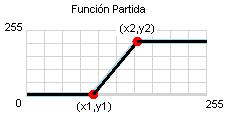
\includegraphics[scale=1.0]{images/funcion_partida.jpg}
	\caption{GUI FUNCION PARTIDA}
	\label{Fig:FunPartida}
\end{figure}

Las funciones \textit{lineal} y \textit{lineal invertida} podr�an representarse con $\{(0;0),(255;255)\}$ y $\{(255;255),(0;0)\}$.

Algo as�:
\begin{figure}
	\centering
	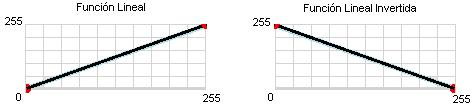
\includegraphics[scale=1.0]{images/funcion_partida_lineal.jpg}
	\caption{GUI FUNCION PARTIDA LINEAL}
	\label{Fig:FunPartidaLineal}
\end{figure}


\subsubsection{Actuadores}

Ahora s�lo nos queda definir los actuadores, su \textit{id} y c�ales \textit{cajas} son sus entradas. El sentido del \textit{id} es igual al que se intenta dar en los sensores, por ejemplo:

Internamente, la salida del \textit{actuador} ser� la sumatoria de todas sus entradas.

\footnotesize	% esto hace que el verbatim se vea chiquitito
\begin{verbatim}
          <actuador id='motor.izquierda'>
            <entradas>
              <entrada id='caja1'/>
              <entrada id='caja2'/>
            </entradas>
          </actuador>

          <actuador id='motor.derecha'>
            <entradas>
              <entrada id='caja2'/>
            </entradas>
          </actuador>
\end{verbatim}
\normalsize	% esto termina el verbatim se vea chiquitito

\subsubsection{Importante}

Las etiquetas y atributos definidos anteriormente deben ser estrictamente definidos de esa forma
en el \textit{XML} (en min�sculas). \textbf{Cualquier otra etiqueta o atributo distintos de:}
\footnotesize	% esto hace que el verbatim se vea chiquitito
\begin{verbatim}
        <ejecucion></ejecucion>
            <sensores></sensores>
                <sensor id='?'/>
            <cajas></cajas>
                <caja></caja>
                    <entradas></entradas>
                        <entrada id='?'/>
                    <puntos>
                        <punto x='?' y='?'/>
            <actuadores></actuadores>
                <actuador></actuador>
                    <entradas></entradas>
                        <entrada id='?'/>
\end{verbatim}
\normalsize	% esto termina el verbatim se vea chiquitito
\textbf{ser�n ignorados.}




\section{GUI Implementaci\'on}
\subsection{Datos para la GUI}

% #############################
\chapter{Log}
\label{cap:log}
%%%%%%%%%%%%%%%%%%%%%%%%%%%%%%%%%%%%%%%%%%%%%%%%%%%%%%%%%%%%
%% LOG
%%%%%%%%%%%%%%%%%%%%%%%%%%%%%%%%%%%%%%%%%%%%%%%%%%%%%%%%%%%%


\section{Introducci\'on}

El archivo de \textit{log} de cada ejecuci�n se encarga de esribirlo el \textit{Core}.
Siempre sobreescribe el archivo especificado, o lo crea si no existe, es decir, s�lo queda en el archivo el contenido de la �ltima ejecuci�n.

El \textit{log} tiene la siguiente especificaci�n:
\begin{enumerate}
 \item \textbf{La primera l�nea.} Consiste de la secuencia, separada por comas, de los \textit{ids} de la tabla de ejecuci�n en el orden en que se encuentran en la misma.
 \item \textbf{Siguientes l�neas.} Son todas iguales. Consiste de varios valores, separados por comas, de la siguiente forma:
	\begin{itemize}
	\item \textit{TimeStamp}. Es el tiempo en \textit{milisegundos} para cada l�nea relativo al comienzo, es decir, comienza en cero.
	\item \textit{Valor de los elementos}. En el mismo orden en que fueron detallados en la primera l�nea, 
		  si es una \texttt{caja} son los valores \textit{entrada} y \textit{salida} de la caja, y si es un \textit{sensor} o un \textit{actuador} es simplemente el valor de \textit{salida}.
	\end{itemize}
\end{enumerate}

Por ejemplo, el siguiente archivo de \textit{log} corresponde a 10 ejecuciones del \textit{Core}:
\footnotesize	% esto hace que el verbatim se vea chiquitito
\begin{verbatim}
        sonar.0, sonar.1, sonar.2, actuador.0, caja.0, caja.1, actuador.1, 
        0, 6, 8, 7, 8, 22, 13, 8, -9, 20, 
        103, 3, 7, 6, 7, 17, 13, 7, -8, 19, 
        204, 8, 3, 2, 3, 14, 13, 3, -6, 15, 
        304, 7, 4, 10, 4, 15, 13, 4, -6, 23, 
        405, 7, 3, 7, 3, 13, 13, 3, -6, 20, 
        505, 10, 8, 9, 8, 26, 13, 8, -9, 22, 
        606, 4, 3, 1, 3, 10, 13, 3, -6, 14, 
        707, 3, 10, 6, 10, 23, 13, 10, -13, 19, 
        807, 8, 10, 9, 10, 28, 13, 10, -13, 22, 
        1009, 3, 2, 7, 2, 7, 8, 2, -6, 15, 
\end{verbatim}
\normalsize	% esto termina el verbatim se vea chiquitito


\textbf{PENDIENTE}

REPLAY Y DEBUG...


\section{Core Implementaci\'on}




% #############################
\chapter{Software adicional}
\label{cap:softadd}
%%%%%%%%%%%%%%%%%%%%%%%%%%%%%%%%%%%%%%%%%%%%%%%%%%%%%%%%%%%%
%% SOFTWARE ADICIONAL
%%%%%%%%%%%%%%%%%%%%%%%%%%%%%%%%%%%%%%%%%%%%%%%%%%%%%%%%%%%%

\section{Xerces XML Parser}
FALTA PONER UNA INTRO!!!

\subsection{Compilaci\'on}
\subsubsection{Linux 32 bits - Librer�as Est�ticas}
El c�digo fuente del Core se compila incluyendo las librer�as est�ticas del Xerces para
que est�n incluidas en el ejecutable del Core y no sea necesario transportalas.
Para eso, es necesario obtener el c�digo fuente de las librer�as del Xerces y recompilarlas de forma est�tica
antes de poder compilar el Core.

Para recompilar las librer�as del Xerces de forma est�tica, los pasos son los siguientes:
\begin{enumerate}
 \item Bajar el archivo \texttt{xerces-c-3.0.1.zip} del c�digo fuente del Xerces de \url{http://apache.xmundo.com.ar/xerces/c/3/sources/xerces-c-3.0.1.zip}
 \item Descomprimir el archivo \texttt{xerces-c-3.0.1.zip} en alguna carpeta, por ejemplo, en \textit{/home/.../workspace/xerces-c-3.0.1-static/}
 \item En la carpeta \textit{/home/.../workspace/xerces-c-3.0.1-static/xerces-c-3.0.1/} ejecutar ``\textit{./configure --disable-shared --disable-network}''
		para que no compile las librer�as din�micas (\textit{.so}), y s�lo compile las est�ticas (\textit{.a}). La opci�n \textit{--disable-network} podr�a obviarse.
 \item En la carpeta \textit{/home/.../workspace/xerces-c-3.0.1-static/xerces-c-3.0.1/} ejecutar ``\textit{make}'' para compilar.
 \item En la carpeta \textit{/home/.../workspace/xerces-c-3.0.1-static/xerces-c-3.0.1/} ejecutar ``\textit{sudo make install}'' para instalar
		las librer�as est�ticas en el sistema. Por defecto, las mismas se instalan en \textit{/usr/local/bin}, \textit{/usr/local/lib}, \textit{/usr/local/include}.
\end{enumerate}

Por �ltimo, para compilar cualquier c�digo fuente que incluya las librer�as, es necesario indicarle al \textit{linker} que
incluya las librer�as est�ticas \textit{/usr/local/lib/libxerces-c.a} y \textit{libpthread.a}. Si esto �ltimo se hace
desde alguna IDE de programaci�n en \texttt{C++} simplemente se agrega en las opciones del programa, \textit{Secci�n Linker}, la
inclusi�n de las librer�as mencionadas. Si la compilaci�n se realiza manualmente, los par�metros son los siguientes:
\texttt{g++ -static -o nombreEjecutable Codigo.cpp -lxerces-c -lpthread}

\subsubsection{Windows 32 bits - Librer�as Est�ticas}
Para recompilar las librer�as del Xerces de forma est�tica en \textit{Windows}, los pasos son los siguientes:

FALTA COMPLETAR ESTO!!!\\FALTA COMPLETAR ESTO!!!\\FALTA COMPLETAR ESTO!!!


\subsection{Compiladores}
\subsubsection{C++ Linux 32 bits}
Utilizamos los siguientes compiladores para C++:
\begin{itemize}
 \item gcc: GCC (GNU Compiler Collection) C compiler.
 \item g++: GCC (GNU Compiler Collection) C++ compiler.
\end{itemize}
Ver \url{http://gcc.gnu.org/}

\subsubsection{C++ Windows 32 bits}
FALTA COMPLETAR ESTO!!!\\FALTA COMPLETAR ESTO!!!\\FALTA COMPLETAR ESTO!!!\\
FALTA COMPLETAR ESTO!!! Para que los comandos como \textit{gcc}, \textit{g++}, \textit{make} (\textit{mingw32-make}) anden en la consola de windows, es necesario modificar la variable de sistema \texttt{PATH} de Windows y agregar la ruta \url{C:/MinGW/bin}.

FALTA COMPLETAR ESTO!!! Ojo con esto, porque aunque simula el GNU-GCC, no necesariamente todas las librer�a incluidas andan, porque algunas son especificas de
Linux, por ejemplo ``sys/socket.h'', que me parece que en Windows hay que cambiarla por ``winsock.h'0'.
HAY QUE VER BIEN ESTO y ANOTAR !!!!

FALTA COMPLETAR ESTO!!! Nota: cualquier cosa, probar tambi�n Cygwin 5.1.6 (GNU + Cygnus + Windows) que contiene de \url{http://www.cygwin.com/}. ojo con esto porque me parece que s� o s� necesita ``cygwin1.dll'' en la PC para que despu�s pueda andar... Probar!!!



\section{YAKS}
YAKS es un simulador de c��digo abierto, escrito en \texttt{C++}, de robots tipo \texttt{Khepera}, desarrollado por Johan Carlsson.
Su nombre proviene del acr�nimo \textit{Yet Another Khepera Simulator}. Posee las siguientes caracter�sticas:
\begin{itemize}
 \item Permite incluir en el entorno obst�culos circulares, paredes, luces y definir zonas.
 \item Permite definir y manipular un n�mero ilimitado de robots.
 \item Permite separar el programa de control del simulador, ya que los robots pueden ser manejados a trav�s de una conexi�n \texttt{TCP/IP}.
 \item Soporta una gran variedad de sensores: proximidad, luminosidad, energ�a, encoders de las ruedas, comp�s y sensor de tierra (para detecci�n de zonas).
\end{itemize}

PONER UNA IMAGEN DEL YAKS!!!!!


\subsection{Ejecuci�n}
\subsubsection{Linux 32 bits}
El YAKS debe ejecutarse manualmente cada vez que se quiera utilizar com RAL desde la GUI. El YAKS se ejecuta de la siguiente forma: \textit{gsim yaks-params.opt}. Debido a que es necesario setear par\'ametros, tanto para el YAKS en \textit{yaks-params.opt} como en el sistema operativo para la librer\'ia GTK, se proporciona un script que tiene en cuenta estos detalles.
\paragraph{Script}
Para facilitar esta ejecuci\'on, se incluye un archivo script \textit{ERBPI/bin/yaks/yaks\_ejecutar.sh}.


Una vez compilado el \textit{YAKS}, podemos proceder a su ejecuci�n. Antes se deber�n realizar las siguientes tareas:
\begin{itemize}
 \item Copiar el ejecutable \textit{gsim} del \textit{YAKS} (que en la compilaci�n fue creado en \textit{src/bin}) en la carpeta ra�z de los fuentes \textit{src}.
 \item Crear el archivo \texttt{yaks-params.opt} de par�metros para la ejecuci�n del \textit{YAKS} en la carpeta ra�z del \textit{YAKS}.
		Puede verse un ejemplo de este archivo en \url{http://www.exa.unicen.edu.ar/catedras/irobotic/yaks-params.htm}. \\
		Es necesario tener en cuenta que la mayor�a de estos ejemplos se encuentran hechos para Windows, por lo tanto es necesario editar todas las rutas
		de archivos y carpetas de ``$.\backslash$'' a ``$./$'' para que funcione correctamente en Linux. Por ejemplo, en el archivo de par�metros de ejemplo, 
		es necesario cambiar ``\texttt{WORLD\_PATH .$\backslash$worlds}'' por ``\texttt{WORLD\_PATH ./worlds}''.
 \item Agregar en el archivo \texttt{yaks-params.opt} de par�metros la l�nea \texttt{CAMERA\_PATH ./cam} para que el \textit{YAKS} sepa d�nde buscar estos archivos.
 \item Ejecuci�n: ejecutar el simulador \textit{YAKS} como \texttt{./gsim yaks-params.opt} en la carpeta ra�z del \textit{YAKS}.
\end{itemize}

\paragraph{Errores en la Ejecuci�n}
Es muy posible que al intentar ejecutar, la librer�a \textit{GTK} arroje errores de ejecuci�n como \texttt{Gdk-ERROR}.

En Linux, esto se debe a que la librer�a \textit{GTK} necesita que los efectos visuales de pantalla del sistema operativo est�n deshabilitados.

En Windows, HAY PROBLEMAS ???  FALTA COMPLETAR ESTO!!!

\textbf{Soluci�n:} Para deshabilitar los efectos visuales, se ejecuta en la consola el comando: \\ \texttt{export XLIB\_SKIP\_ARGB\_VISUALS=1}

\subsubsection{Windows 32 bits}
FALTA COMPLETAR ESTO!!!\\FALTA COMPLETAR ESTO!!!\\FALTA COMPLETAR ESTO!!!\\


\subsection{Compilaci�n}

COMPLETAR ESTO CON \url{http://profesores.elo.utfsm.cl/~tarredondo/memorias/2005-memoria-fquiros.pdf} QUE EXPLICA MUUY BIEN TODO EL YAKS...


\label{YAKSCompilacion}
El c�digo fuente del YAKS se encuentra en \url{http://www.exa.unicen.edu.ar/catedras/irobotic/YAKS.htm} En particular, bajamos dos archivos:
\begin{itemize}
 \item \url{http://www.exa.unicen.edu.ar/catedras/irobotic/SOFTWARE/YAKS-src-update-2.zip}: C�digo Fuente Completo para Linux.
 \item \url{http://www.exa.unicen.edu.ar/catedras/irobotic/SOFTWARE/yaks-linux-patch.tar.gz}: Patch de YAKS para que no tire errores al compilarlo en Unix.
\end{itemize}

Luego se descomprime el contenido de los dos archivos fuentes en alguna carpeta, por ejemplo \texttt{yaks/src}.

\subsection{Linux 32 bits}

\begin{itemize}
 \item En la carpeta donde se encuentra el c�digo fuente del \textit{YAKS}, creamos dos carpetas \textit{bin} y \textit{lib},
		que son necesarias para crear los archivos resultantes de la compilaci�n.
 \item Instalar la librer�a \textit{GTK}, que es una librer�a estandard de \texttt{C++} para el manejo de ventanas gr�ficas.
	  Se puede instalar de la siguiente forma: \texttt{sudo apt-get install libgtk1.2-dev}
 \item Compilar: en la carpeta donde se encuentra el c�digo fuente del \textit{YAKS}, ejecutar \texttt{make}
\end{itemize}

\subsubsection{Errores en la Compilaci�n}
Es muy posible que al intentar compilar, el compilador arroje errores relacionados con \texttt{iostream.h}, \texttt{cout} y \texttt{endl} en los archivos fuentes
\texttt{ann.cpp}, \texttt{ann.h}, \texttt{ga.cpp} y \texttt{ga.h}.

En Linux, este problema se origina al enlazar con la librer�a \textit{GTK}, ya que no es posible utilizar \texttt{std::cout}
porque no ``entiende'' a qu� pantalla o consola tiene que mandar el \textit{stream}, puesto que la librer�a \textit{GTK} maneja varias pantallas.

\textbf{Soluci�n:} Es necesario editar los archivos fuentes \texttt{ann.h}, \texttt{ann.cpp} y \texttt{ga.h}, sacando de los mismos las l�neas
\texttt{\#include<iostream.h>} y \texttt{std::cout} (con sus respectivos operadores $<<$). Si se deseara mantener la impresi�n por pantalla, se deber�an cambiar los
\texttt{std::cout} por la funci�n \texttt{printf} de \texttt{C}.

\subsubsection{Error de Librer\'ia GTK}

Al parecer, la librer�a \textit{libgtk1.2-dev} est\'a desactualizada (muy vieja) y no est\'a m\'as disponible en los repositorios de Ubuntu.
La opci�n que queda es instalar la \textit{libgtk2.0-dev}. Pero con esta nueva versi�n, el YAKS da errores de compilaci\'on.

\textbf{Soluci\'on 1:} Agregar en la lista de fuentes del \textit{apt} el lugar desde donde bajar la \textit{libgtk1.2-dev}, as�:
\begin{verbatim}
        sudo gedit /etc/apt/sources.list
\end{verbatim}
agregar al final la l�nea ``\textit{deb http://cz.archive.ubuntu.com/ubuntu hardy main universe}'' y ejecutar:
\begin{verbatim}
        sudo apt-get update
        sudo apt-get install libgtk1.2-dev
\end{verbatim}
ahora deber\'ia instalarse autom\'aticamente.

Si no anda, es necesario bajar y compilar a mano la librer�a desde: \url{http://packages.ubuntu.com/hardy/i386/libgtk1.2-dev/download}.

\textbf{Soluci\'on 2:} Corregir los fuentes del YAKS para que compile con la \textit{libgtk2.0-dev}. Parece complicado... ESTO EST\'A PENDIENTE !!!!

Y HAY QUE HCERLO PORQUE EN LOS LABOS NO DAN MAS SOPORTE PARA \textit{libgtk1.2-dev}, S\'OLO VAN A TENER LA \textit{libgtk2.0-dev} !!!! HABLAR COM Maximiliano Geier !!!

\subsubsection{Script}
Para facilitar la compilacion, se incluye un archivo script ``yaks\_compilar.sh''. El mismo puede ejecutar simplemente con \texttt{./yaks\_compilar.sh}.


\subsection{Windows 32 bits}

FALTA COMPLETAR ESTO!!! Nota: cualquier cosa, probar tambi�n Cygwin 5.1.6 (GNU + Cygnus + Windows) que contiene de \url{http://www.cygwin.com/}. ojo con esto porque me parece que s� o s� necesita ``cygwin1.dll'' en la PC para que despu�s pueda andar... Probar!!!



\subsection{YAKS para Windows 32 bits}

FALTA COMPLETAR ESTO!!!\\
FALTA COMPLETAR ESTO!!!

\subsection{Instalaci\'on}
\subsubsection{Linux 32 bits}
Para la instalaci\'on se ejecuta el script \textit{ERBPI/src/yaks/yaks\_instalar.sh}. Es necesario que el YAKS se encuentre compilado con anterioridad. Para compilaci\'on de YAKS ver punto \ref{YAKSCompilacion}.
\subsubsection{Windows 32 bits}
FALTA COMPLETAR ESTO!!!\\FALTA COMPLETAR ESTO!!!\\FALTA COMPLETAR ESTO!!!\\




\subsection{Compiladores}
\subsubsection{C++ Linux 32 bits}
Utilizamos los siguientes compiladores para C++:
\begin{itemize}
 \item gcc: GCC (GNU Compiler Collection) C compiler.
 \item g++: GCC (GNU Compiler Collection) C++ compiler.
\end{itemize}
Ver \url{http://gcc.gnu.org/}

\subsubsection{C++ Windows 32 bits}
FALTA COMPLETAR ESTO!!!\\FALTA COMPLETAR ESTO!!!\\FALTA COMPLETAR ESTO!!!\\
FALTA COMPLETAR ESTO!!! Para que los comandos como \textit{gcc}, \textit{g++}, \textit{make} (\textit{mingw32-make}) anden en la consola de windows, es necesario modificar la variable de sistema \texttt{PATH} de Windows y agregar la ruta \url{C:/MinGW/bin}.

FALTA COMPLETAR ESTO!!! Ojo con esto, porque aunque simula el GNU-GCC, no necesariamente todas las librer�a incluidas andan, porque algunas son especificas de
Linux, por ejemplo ``sys/socket.h'', que me parece que en Windows hay que cambiarla por ``winsock.h'0'.
HAY QUE VER BIEN ESTO y ANOTAR !!!!

FALTA COMPLETAR ESTO!!! Nota: cualquier cosa, probar tambi�n Cygwin 5.1.6 (GNU + Cygnus + Windows) que contiene de \url{http://www.cygwin.com/}. ojo con esto porque me parece que s� o s� necesita ``cygwin1.dll'' en la PC para que despu�s pueda andar... Probar!!!


\section{SimuladorExaBot}


% #############################
\chapter{Compilaci\'on, Instalaci\'on y Ejecuci\'on}
\label{cap:CompInstExec}
%%%%%%%%%%%%%%%%%%%%%%%%%%%%%%%%%%%%%%%%%%%%%%%%%%%%%%%%%%%%
%% COMPILACION, INSTALACION Y EJECUCION
%%%%%%%%%%%%%%%%%%%%%%%%%%%%%%%%%%%%%%%%%%%%%%%%%%%%%%%%%%%%

\section{Compilaci\'on}

\section{Instalaci\'on}
Estructuralmente el software se divide en dos carpetas:
\begin{enumerate}
 \item \textbf{\textit{ERBPI/src:}} contiene todos los fuentes necesarios del software para su compilaci\'on.
 \item \textbf{\textit{ERBPI/bin:}} contiene todos los ejecutables, producto de la compilasi\'on de los fuentes, necesarios para la ejecuci\'on completa del software.
\end{enumerate}

Cada m\'odulo y RALs contienen su fuentes y, por lo tanto, sus scripts necesarios para su compilacion e instalaci\'on. La instalaci\'on de cada m\'odulo produce la estructura de binarios siguientes:
\begin{itemize}
 \item ERBPI/bin:
  \begin{itemize}
    \item /core
    \item /gui
    \item /yaks
  \end{itemize}
\end{itemize}

Opcionalmente tambi\'en se introduce en la carpeta \textit{ERBPI/bin/comportamientos} que contiene archivos \textit{XML} con comprtamientos est\'andard ya programados.


\section{Ejecuci\'on}

% #############################
% 	\appendix
% 	\chapter{Ap\'endice}
\label{chap:apendice1}

\section{BlaAp1}

asdas sad
sad
sad
asd

And I cite myself to show by bibtex style file (two authors) \cite{Commowick_MICCAI_2007}.

This for other bibtex stye file : only one author \cite{Oakes_RStat_1999} and many authors \cite{Guimond_CVIU_2000}.
% #############################
%  	\bibliographystyle{template/ThesisStyle}
% 	\bibliography{bibliografia}

% #############################
\chapter{Bugs}
\label{cap:bugs}
%%%%%%%%%%%%%%%%%%%%%%%%%%%%%%%%%%%%%%%%%%%%%%%%%%%%%%%%%%%%
%% BUGS
%%%%%%%%%%%%%%%%%%%%%%%%%%%%%%%%%%%%%%%%%%%%%%%%%%%%%%%%%%%%

Estos son bugs conocidos, algunos arreglados y otro no...

% \section{BUGs}

\section{Sin Arreglar}

\subsection{Khepera RAL}
\label{bugSA01}
A veces el KHEPERA-RAL no arranca, tira  \texttt{segmentation fault}... Parece ser un problema de que no puede abrir bien el puerto COM... Hay que darle hasta que deje de devolver \texttt{segmentation fault}...

\subsection{Khepera RAL Torreta-Radio}
\label{bugSA02}
Parece haber un problema con el \textit{setMotors(motors)} en \textit{setEstadoActuadores()} en el \textit{RAL.CPP}. Si comentamos esto, la lectura de sensores a \textit{CTR\_FREC = 700000} anda b\'arbaro, si no, empieza a fallar...

El error t\'ipico parece ser que se pierden lecturas y devuelve todo cero. 
Una salida de log t\'ipica cuando est\'a activado el \textit{setMotors(motors)} de la funci�n \textit{setEstadoActuadores()} en \textit{RAL.CPP} es:

\scriptsize
\begin{verbatim}
timestamp, proximidad.320, proximidad.340, proximidad.350, proximidad.10, proximidad.20, proximidad.40, proximidad.170, proximidad.190, funcion.exitatoria.1, funcion.exitatoria.2, funcion.inhibitoria.1, funcion.inhibitoria.2, motor.izquierda, motor.derecha, 
0, 0, 0, 0, 0, 0, 0, 0, 0, 0, 3, 0, 3, 0, 0, 0, 0, 3, 3, 
701, 1023, 1023, 141, 0, 0, 0, 0, 0, 2187, 10, 0, 3, 0, 0, 2187, -10, 10, -7, 
1402, 0, 0, 0, 0, 0, 0, 0, 0, 0, 3, 0, 3, 0, 0, 0, 0, 3, 3, 
2103, 0, 0, 0, 0, 0, 0, 0, 0, 0, 3, 0, 3, 0, 0, 0, 0, 3, 3, 
2804, 0, 0, 0, 0, 0, 0, 0, 0, 0, 3, 0, 3, 0, 0, 0, 0, 3, 3, 
3505, 1023, 1023, 393, 0, 0, 0, 0, 0, 2439, 10, 0, 3, 0, 0, 2439, -10, 10, -7, 
4206, 0, 0, 0, 0, 0, 0, 0, 0, 0, 3, 0, 3, 0, 0, 0, 0, 3, 3, 
4907, 0, 0, 0, 0, 0, 0, 0, 0, 0, 3, 0, 3, 0, 0, 0, 0, 3, 3, 
5607, 0, 0, 0, 0, 0, 0, 0, 0, 0, 3, 0, 3, 0, 0, 0, 0, 3, 3, 
6307, 1023, 1023, 603, 0, 0, 0, 0, 0, 2649, 10, 0, 3, 0, 0, 2649, -10, 10, -7, 
7008, 0, 0, 0, 0, 0, 0, 0, 0, 0, 3, 0, 3, 0, 0, 0, 0, 3, 3, 
7710, 0, 0, 0, 0, 0, 0, 0, 0, 0, 3, 0, 3, 0, 0, 0, 0, 3, 3, 
8410, 0, 0, 0, 0, 0, 0, 0, 0, 0, 3, 0, 3, 0, 0, 0, 0, 3, 3, 
9111, 1023, 1023, 244, 0, 0, 0, 0, 0, 2290, 10, 0, 3, 0, 0, 2290, -10, 10, -7, 
\end{verbatim}
\normalsize

En cambio, si lo comentamos empieza a andar todo bien:

\scriptsize
\begin{verbatim}
timestamp, proximidad.320, proximidad.340, proximidad.350, proximidad.10, proximidad.20, proximidad.40, proximidad.170, proximidad.190, funcion.exitatoria.1, funcion.exitatoria.2, funcion.inhibitoria.1, funcion.inhibitoria.2, motor.izquierda, motor.derecha, 
0, 0, 0, 0, 0, 0, 0, 0, 0, 0, 3, 0, 3, 0, 0, 0, 0, 3, 3, 
702, 677, 1023, 0, 0, 0, 0, 0, 0, 1700, 10, 0, 3, 0, 0, 1700, -10, 10, -7, 
1403, 1023, 1023, 292, 0, 0, 0, 0, 0, 2338, 10, 0, 3, 0, 0, 2338, -10, 10, -7, 
2103, 1023, 1023, 136, 0, 0, 0, 0, 0, 2182, 10, 0, 3, 0, 0, 2182, -10, 10, -7, 
2804, 1023, 1023, 170, 0, 0, 0, 0, 0, 2216, 10, 0, 3, 0, 0, 2216, -10, 10, -7, 
3504, 1023, 1023, 102, 0, 0, 0, 0, 0, 2148, 10, 0, 3, 0, 0, 2148, -10, 10, -7, 
4205, 1023, 1023, 174, 0, 0, 0, 0, 0, 2220, 10, 0, 3, 0, 0, 2220, -10, 10, -7, 
4905, 1023, 1023, 330, 0, 0, 0, 0, 0, 2376, 10, 0, 3, 0, 0, 2376, -10, 10, -7, 
5605, 1023, 1023, 261, 0, 0, 0, 0, 0, 2307, 10, 0, 3, 0, 0, 2307, -10, 10, -7, 
6306, 1023, 1023, 180, 0, 0, 0, 0, 0, 2226, 10, 0, 3, 0, 0, 2226, -10, 10, -7, 
7707, 1023, 1023, 144, 0, 0, 0, 0, 0, 2190, 10, 0, 3, 0, 0, 2190, -10, 10, -7, 
8407, 1023, 1023, 245, 0, 0, 0, 0, 0, 2291, 10, 0, 3, 0, 0, 2291, -10, 10, -7, 
9108, 1023, 1023, 125, 0, 0, 0, 0, 0, 2171, 10, 0, 3, 0, 0, 2171, -10, 10, -7, 
9808, 845, 1023, 0, 0, 0, 0, 0, 0, 1868, 10, 0, 3, 0, 0, 1868, -10, 10, -7, 
10508, 1023, 1023, 0, 0, 0, 0, 0, 0, 2046, 10, 0, 3, 0, 0, 2046, -10, 10, -7, 
11209, 1023, 1023, 0, 0, 0, 0, 0, 0, 2046, 10, 0, 3, 0, 0, 2046, -10, 10, -7, 
11909, 1023, 1023, 33, 0, 0, 0, 0, 0, 2079, 10, 0, 3, 0, 0, 2079, -10, 10, -7, 
\end{verbatim}
\normalsize

\subsection{GUI Reseteo Workbench}
\label{bugSA03}

\textbf{Pregunta:} �Se puede ejecutar el mismo comportamiento en dos robots diferentes? Por ejemplo, si s�lo 
usas telemetros en el Exabot para evitar obstaculos, podes pasar el mismo comportamiento al Khepera? �D�nde 
est� la normalizacion de los sensores, en el RAL? 
\textbf{Respuestas:}
\begin{itemize}
\item La normalizaci�n de sensores est� en RAL, entonces se podr�an reutilizar los comportamientos para distintos robots porque todo pasa a ser relativo a 0-100\%.
\item Reutilizar comportamiento en disntintos robots: Objetivamente s� se puede. Pero en realidad, como no tuve tiempo de ``tocarlo bien'' en el c�digo de Java, cuando cambi�s en el men� de la GUI de selecci�n de robot, te resetea el ``escritorio de trabajo'' (workbench) de la GUI... Es s�lo un problemita menor de programaci�n en la GUI... S�lo habr�a que tocar la GUI para que no resetee el workbench y vuele los sensores y actuadores (con sus conexiones) que no corresponden en funci�n del nuevo robot...
\end{itemize}

Si programaste un comportamiento y cambi\'as el robot desde el menu de selecci\'on de robot, se reseteo todo!!! ARREGLAR ESTO!!!

Ver Bug Arreglado en \ref{bugA02}

\subsection{GUI lectura componentes - sensores}
\label{bugSA04}
Hay 2 problemas: por c\'omo hice el c�digo de la GUI en \textit{JRobotPanel::JSensorsChooserDialog()} los IDs de los sensores deben ser \texttt{tipo.numero}. Si lo que est� despu�s del punto no es un n�mero, no anda. Si lo que est� antes del punto no es igual a unp de los \texttt{tipo}, no anda. Entonces, el formato debe ser: 
\scriptsize
\begin{verbatim}
                <sensor id='telemetro.45' tipo='telemetro'>
\end{verbatim}
\normalsize

\subsection{RAL ExaBot}
\label{bugSA05}
Falta hacer una funci\'on \texttt{inicializarRAL(lista sensores)} para que prenda s�lo algunos sensores, los pasados por la lista. El problema es que por defecto la RAL prende todos los sensores del robot. Cuando esto no es necesario, tener todos los sensores prendidos consume mucha energ\'ia y las bater\'ias del robot se gastan muy r\'apido.

Esto es principalmente para el Exabot, pero hay que dejarla establecida en el \texttt{.H} para todas las RALs...


\subsection{GUI}
\label{bugSA06}
Abrir la gui no maximizada. 
Abrir la pantalla de seleccion de robot. 
Maximizar la ventana. 
La pantalla queda de tama�o chiquito!!







%%%%%%%%%%%%%%%%%%%%%%%%%%%%%%%%%%%%%%%%%%%%%%%%%%%%%%%%%%%%%%%%%%%%%%%%%%%%%%%%%%%%%%%%%%%%%%%%%%%%%%%%%%%%%%%%
%%%%%%%%%%%%%%%%%%%%%%%%%%%%%%%%%%%%%%%%%%%%%%%%%%%%%%%%%%%%%%%%%%%%%%%%%%%%%%%%%%%%%%%%%%%%%%%%%%%%%%%%%%%%%%%%
\section{Arreglados}

\subsection{GUI Ejecuci\'on}
\label{bugA01}
Tenemos un problema, despu�s de darle ejecutar a la GUI (por ejemplo con el YAKS) el yaks se cerraba solo a los 10 segundos... El problema era que el applet (ventanita) de la GUI que indicaba que se estaba ejecutando (el CORE) no freezaba (deten�a) la ejecuci�n de la GUI, entonces inmediatamente lo que segu\'ia a ejecutar era el \texttt{proc.destroy()} en la GUI. A esto se le sumaba que el \texttt{proc.destroy()} a veces no mataba bien el proceso y quedaba pululando el CORE por ah\'i y empezaba a andar todo mal!!! imaginate dos COREs corriendo al mismo tiempo!!!...

No pudimos arreglar bien esto y por falta de tiempo lo EMPARCHAMOS horriblemente haciendo que el Java se freeze con una ventanita esperando el bot\'on STOP y cuando se presione inmediatamente busque el IDPROC del CORE y mande \texttt{killall} via sistema para matar el CORE. ESTO ES HORRIBLE!!!! OJO!!! Esto s\'olo anda en LINUX!!!! Para que termine bien el CORE con SIGINT (Ctrl+C) lo arreglamos as\'i:
\scriptsize
\begin{verbatim}
                kill -2 pid
                ps -ef
                kill -int pid
\end{verbatim}
\normalsize
el pid tiene que ser el de
\scriptsize
\begin{verbatim}
                -> /lib/ld-linux.so.2 --library-path ../core ../core/core_exe /tmp/prg-4851298914852602110 core_log.txt yaks
\end{verbatim}
\normalsize
y no el de
\scriptsize
\begin{verbatim}
                   /bin/sh ../core/core.sh /tmp/prg-4851298914852602110 core_log.txt yaks
\end{verbatim}
\normalsize
con 
\scriptsize
\begin{verbatim}
                   ps -ef | grep /lib/ld
\end{verbatim}
\normalsize
obtengo listada s�lo la linea del proceso que me interesa:
\scriptsize
\begin{verbatim}
                javier    8933  8932  0 17:52 ?        00:00:00 /lib/ld-linux.so.2 --library-path ../core ../core/core_exe /tmp/prg-3610233313880776518 core_log.txt yaks	
\end{verbatim}
\normalsize
entonces la segunda ``palabra'' es el pid que me interesa...

Puede verse m\'as en: \url{http://www.devdaily.com/java/edu/pj/pj010016}, \url{http://bugs.sun.com/bugdatabase/view_bug.do?bug_id=4784574}, \url{http://ubuntuforums.org/showthread.php?t=995619}, \url{http://www.experts-exchange.com/Programming/Languages/Java/Q_22052834.html}.

Al final, lo solucion\'e haciendo lo diguiente:
\scriptsize
\begin{verbatim}
                // obtengo el PID del "core_proc"
                String[] params2 = new String[] { "/bin/bash", "-c",  "ps -ef | grep /lib/ld" };
                Process core_proc_pid = Runtime.getRuntime().exec(params2);
                BufferedReader core_proc_pid_br = new BufferedReader(new InputStreamReader(core_proc_pid.getInputStream()));
                String core_proc_pid_br_line = core_proc_pid_br.readLine();
                StringTokenizer core_proc_pid_br_line_st = new StringTokenizer( core_proc_pid_br_line );
                String core_proc_PID;
                core_proc_PID = core_proc_pid_br_line_st.nextToken();
                core_proc_PID = core_proc_pid_br_line_st.nextToken();
                System.out.println("-> el PID del core es: " + core_proc_PID);

                // termina el core enviando el signal SIGINT // obtengo el PID del "core_proc"
                String[] params3 = new String[] { "/bin/bash", "-c",  "kill -int " + core_proc_PID };
                Process core_proc_SIGINT = Runtime.getRuntime().exec(params3);
                System.out.println("-> hicimos 'kill -int " + core_proc_PID + "' y matamos el core...");
\end{verbatim}
\normalsize

Ahora despu\'es de un tiempo, creo que el problema era que no estaba bien implementado el \texttt{SIGTERM} Y \texttt{SIGINT} en el CORE. Pero esto ya lo arreglamos. Habr\'ia que volver atr\'as esta modificaci\'on y ver que est\'e andando correctamente...

Este moco se encuentra en el archivo \textit{JRoboticaFrame.java}.

\subsection{GUI Menu Selecci\'on Robot}
\label{bugA02}
No andaba bien el menu de cambio de Robot. El problema era que trataba de buscar los XMLs de robots en \textit{extension/robots} y ten�a que buscarlos en \textit{bin/extension/robots} ya que el programa ejecuta desde el directorio \textit{gui} y no desde \textit{gui/bin}...

Adem\'as, para que al cambiar el robot en el menu tambi\'en cambie todo en la aplicaci\'on (se actualice) tambi\'en hubo que tocar lo siguiente:
\begin{itemize}
	\item \verb=JRoboticaFrame::openProgram(File f):= leemos del archivo cu�l es el robot y actualizamos \textit{programPanelHolder}, \textit{robotPanel} y \textit{robotNameLabel.setText(robot.getName())}.
	\item \verb=JRoboticaFrame::actionPerformed(e.getActionCommand().startsWith("changeRobot:")):= actualizamos \textit{robot}, \textit{robotNameLabel}, \textit{programPanelHolder} y \textit{robotPanel}. 
\end{itemize}
\textbf{OJO:} Es decir que, si ten�s un programa armado para un robot y toc�s cambiar el robot, te borra todo y empieza de nuevo, porque no tiene sentido ya que los sensores se llaman distintos!!! ESTO \'ULTIMO NO EST\'A BIEN!!! HAY QUE ARREGLARLO PARA QUE UN COMPORTAMIENTO PUEDA USARSE PARA DISTINTOS ROBOTS!!!! Ver Bug Sin Arreglar en \ref{bugSA03}...


\subsection{GUI Configurar Par\'ametros de Funciones (Cajas)}
\label{bugA03}
Hubo que combinar con c\'odigo Diego para que le pase a \textit{cajaParametros} los 2 puntos para dibujarlos y que al presionar los boton aceptar devuelva a la GUI valor de los 2 puntos modificados...

?`Qu\'e hicimos?

en JBox.java:
\scriptsize
\begin{verbatim}
                        private JPopupMenu getPopupMenu() {
                            ...
                            item2.setActionCommand("setup");
                            popup.add(item);
                            if( box instanceof FunctionBox )
                                popup.add(item2);
                        public void actionPerformed(ActionEvent e) {
                            ...
                            if( e.getActionCommand() == "setup" ) {
                                Point A = new Point();
                                Point B = new Point();
                                A.x = ((FunctionBox) this.box).getX0();
                                A.y = ((FunctionBox) this.box).getY0();
                                B.x = ((FunctionBox) this.box).getX1();
                                B.y = ((FunctionBox) this.box).getY1();
                                JParametrosCaja setupBox = new JParametrosCaja( A,B, Program.getCurrentProgram(), this.box );
                                setupBox.run();
                            }
\end{verbatim}
\normalsize
en FunctionBox.java:
\scriptsize
\begin{verbatim}
                        public void setX0( int valor )...
                        public void setY0( int valor )...
                        public void setX1( int valor )...
                        public void setY1( int valor )...
\end{verbatim}
\normalsize
en ProgramListener.java:
\scriptsize
\begin{verbatim}
                        public interface ProgramListener {
                            public void boxSet( Box box, Point A, Point B );
\end{verbatim}
\normalsize
en Program.java:
\scriptsize
\begin{verbatim}
                        public void setBox( Box box, Point A, Point B ) {        
                            for( ProgramListener listener: listeners )
                                listener.boxSet(box,A,B);        
\end{verbatim}
\normalsize
en JConnectionsPanel.java:
\scriptsize
\begin{verbatim}
                        public void boxSet( Box box, Point A, Point B ){}
\end{verbatim}
\normalsize
en JBoxPanel.java:
\scriptsize
\begin{verbatim}
                        public void boxSet( Box box, Point A, Point B ){
                            if( box instanceof FunctionBox ){
                                ((FunctionBox) box).setX0(A.x);
                                ((FunctionBox) box).setY0(A.y);
                                ((FunctionBox) box).setX1(B.x);
                                ((FunctionBox) box).setY1(B.y);
                            }
                        }
\end{verbatim}
\normalsize
en JParametrosCaja.java:
\scriptsize
\begin{verbatim}
                        public JParametrosCaja( Point puntoA, Point puntoB, Program programa, Box box )...
                        public void actionBotonCerrarAceptar(){
                            this.puntoARet.x = (int)normalizarPunto(punto2).x;
                            this.puntoARet.y = (int)normalizarPunto(punto2).y;
                            this.puntoBRet.x = (int)normalizarPunto(punto3).x;
                            this.puntoBRet.y = (int)normalizarPunto(punto3).y;
                            this.programa.setBox( this.box, puntoARet, puntoBRet );
                            frameVentana.dispose();
                        }

\end{verbatim}
\normalsize


\subsection{GUI bolas de poder (funci\'on constante)}
\label{bugA04}
Si est\'abamos usando la GUI con Yaks-RAL y pon\'iamos al menos 3 ``bolas de energia'' a una rueda, ya no se mueve!!

El problema es que el Yaks (simulador) no acepta m�s de \verb=valor 10= \'o \verb=valor -9= para el motor (adelante \'o atr\'as)... Es decir, si le mando \texttt{10} o \texttt{-9} anda, si le mando \texttt{11} o \texttt{-10} ya no... En valores normalizados (desde la GUI),  para adelante anda hasta valor 54 (54\%), desde 55 en adelante ya deja de andar... Para atr\'as normalizadado anda hasta valor -49 (-49\%), desde -50 en adelante ya deja de andar...

Para arreglar esto, modificamos la funci�n \verb=RAL::desNormalizarMotores()= del Yaks para que sature en los valores antes mencionados.

En el RAL-Khepera no tiene este problema, entonces los valores desnormalizados van entre \texttt{-20:20}, o normalizados entre \texttt{-100\%:100\%}


\subsection{Core Finalizaci\'on}
\label{bugA05}
Hab\'ia problemas con el manejo de se\~nales de finalizaci\'on (\texttt{SIGINT} y \texttt{SIGTERM}) del Core junto con la RAL. Un ejemplo de este problema es los que pasaba en \ref{bugA06}.

Al prinicipio s\'olo atend\'iamos la se\~nal \texttt{SIGINT}. Luego incorpor\'amos la atenci\'on de \texttt{SIGTERM}. La se�al \texttt{SIGINT} (\textit{interrupt key signal}), es una se�al de atenci�n interactiva, generalmente generada por la teclas \texttt{Ctrl+C} en la consola de ejecuci�n, pero que tambi�n puede ser enviada por otro programa. La se�al \texttt{SIGTERM} (\textit{termination signal}), es una se�al de terminaci\'on enviada por el comando \texttt{kill}, pero que tambi�n puede ser enviada por otro programa.

Tambi\'en hab\'ia problemas de entrelazamiento de atenci\'on de se\~nales, en particular con RALs que manejan varios threads como RAL-ExaBot, que hac\'ia que los procesos no terminaran en el orden correcto ni de forma correcta. Para solucionar esto hubo que arreglar varias cosas:
\begin{itemize}
	\item \textbf{Core:} 
		\begin{itemize}
			\item La llamada a la funci\'on \verb=inicializarRAL()= la hacemos lo m\'as arriba posible (o lo m\'as antes posible) para que, en casos como RAL-ExaBot que tiene varios threads, comparta lo menos posible de memoria con el proceso \textit{padre} Core, como ser \textit{fileDescriptors}, etc. De lo contrario aumenta la probabilidad de que sucedan cosas indeseadas.
			\item Tambi\'en por lo anterior, pusimos la llamada a la atenci\'on de se\~nales inmediatamente despu\'es de \verb=inicializarRAL()=, para que la atenci\'on de la se\~nal del Core est\'e separada del haber levantado los procesos necesarios para la RAL. De lo contrario, suced\'ia que inmediatamente la se\~nal era atendida tambi\'en por los procesos de la RAL y en algunos casos, como RAL-ExaBot, esto resultaba en un comportamiento de finalizaci\'on no deseado.
			\item Tambi\'en agregamos para completitud de casos adem\'as de \texttt{SIGINT}, la atenci\'on de la se\~nal \texttt{SIGTERM} para que tambi�n atienda a la se�al del comando de sistema \texttt{kill}.
		\end{itemize}
	\item \textbf{RAL-ExaBot:} ver bugs arreglados en \ref{bugA06}.
\end{itemize}


\subsection{RAL ExaBot Threads-Signals }
\label{bugA06}
Al finalizar el RAL, cuando deten\'iamos la ejecuci\'on del comportamiento desde la GUI, los motores segu\'ian andando, es decir, no les asignaba valor 0 (cero) para detenerlos.

El problema era con el manejo de los procesos \verb=core= (\textit{padre}) y \verb=udp_receive= - \verb=udp_send= (\textit{hijos}).
Al enviar las se\~nales de finalizaci\'on para que el Core las atendiera como \verb=Ctrl+C=, \verb=kill -int Core= o \verb=kill Core= le mandaba la se�al a los 3 procesos (padre y 2 hijos), 
entonces \verb=udp_send= nunca terminaba y nunca llegaba a enviar 0 (cero) a los motores.

Para solucionar esto hubo que arreglar varias cosas:
\begin{itemize}
	\item \textbf{Core:} ver bugs arreglados en \ref{bugA05}.
	\item \textbf{RAL-ExaBot:} 
		\begin{itemize}
			\item Hicimos que los procesos \textit{hijos} (\verb=udp_receive= y \verb=udp_send=) del \textit{padre} RAL-ExaBot (\verb=core=) no dependan de la misma consola, los desatacheamos. Para esto utilizamos el comando de linux \textit{setsid} mediante la funci\'on de C \verb=setsid()=, con lo que desatacheamos el hijo del padre. Es para que el hijo no dependa de la misma consola. Es decir, no muera con el \verb=Ctrl+C=, \verb=kill -int Core= o \verb=kill Core= del padre (Core).\\El comando \textit{setsid} crea una nueva sesi�n para el proceso llamador, quedando como \'unico proceso en este nuevo grupo de procesos.
			\item En \verb=udp_send()= agregamos:
				\scriptsize
				\begin{itemize}
					\item \verb=signal(SIGINT,terminar_udp_send);  // configurar la rutina de atenci�n de SIGINT=
					\item \verb=signal(SIGTERM,terminar_udp_send); // configurar la rutina de atenci�n de SIGTERM=\\
						  \verb=                                   // que no hace nada, pero atiende:=
						  \verb=                                   //     void terminar_udp_send(int sig){exit(sig);}=
				\end{itemize}
				\normalsize
			\item En \verb=udp_receive()= agregamos:
				\scriptsize
				\begin{itemize}
					\item \verb=signal(SIGINT,terminar_udp_receive);  // configurar la rutina de atenci�n de SIGINT=
					\item \verb=signal(SIGTERM,terminar_udp_receive); // configurar la rutina de atenci�n de SIGTERM=\\
						  \verb=                                      // que no hace nada, pero atiende:=
						  \verb=                                      //     void terminar_udp_receive(int sig){exit(sig);}=
				\end{itemize}
				\normalsize
		\end{itemize}
\end{itemize}











% #############################
\chapter{Referencias}
\label{cap:ref}
%%%%%%%%%%%%%%%%%%%%%%%%%%%%%%%%%%%%%%%%%%%%%%%%%%%%%%%%%%%%
%% REFERENCIAS
%%%%%%%%%%%%%%%%%%%%%%%%%%%%%%%%%%%%%%%%%%%%%%%%%%%%%%%%%%%%



% Realizamos un survey de interfaces gr�ficas de programaci�n.
% 
% Estos son todos proyectos para ni�os, la mayor�a implementados para la OLPC (One Laptop Per Child Project):
% \begin{itemize}
%   \item StarLogo TNG \\ \url{http://education.mit.edu/drupal/starlogo-tng}
%   \item EToys (Smalltalk/Squeak) \\ \url{http://wiki.laptop.org/go/Etoys} \\ \url{http://www.squeakland.org/download/}
%   \item Scratch (Squeak) \\ \url{http://scratch.mit.edu/}
% \end{itemize}
% 
% Tambi�n hay un framework de Microsoft:
% \begin{itemize}
%   \item Microsoft Robotics Developer Studio (RDS)\\ \url{http://msdn.microsoft.com/en-us/library/cc998476.aspx}
% 	\item Microsoft Visual Programming Language (VPL) \\ \url{http://msdn.microsoft.com/en-us/library/bb483088.aspx}
% 	\item Microsoft Visual Simulation Environment (VSE) \\ \url{http://msdn.microsoft.com/en-us/library/bb483076.aspx}
% \end{itemize}

\begin{thebibliography}{9}
	\bibitem{xml} \textit{XML: Extensible Markup Language}. ????????????? \url{http://?????????????????}.

	\bibitem{dom} \textit{DOM: Document Object Model}. \url{http://xerces.apache.org/xerces-c/api-3.html}, \url{http://www.w3.org/DOM}.

	\bibitem{kheperaDoc} \textit{Khepera Documentation}. \url{http://ftp.k-team.com/khepera/documentation}.

	\bibitem{kheperaManual} \textit{Khepera User Manual}. \url{http://ftp.k-team.com/khepera/documentation/KheperaUserManual.pdf}.

	\bibitem{kheperaBase} \textit{Khepera Radio Base User Manual}. \url{http://ftp.k-team.com/khepera/documentation/RadioBaseManual.pdf}.

	\bibitem{kheperaTurret} \textit{Khepera Radio Turret User Manual}. \url{http://ftp.k-team.com/khepera/documentation/RadioTurretManual.pdf}.

	\bibitem{signals} \textit{The C Book: Signal handling}. \url{http://publications.gbdirect.co.uk/c_book/chapter9/signal_handling.html}.







 	\bibitem{pyro} \textit{Pyro: A python-based versatile programming environment for teaching robotics}. D.S. Blank, D. Kumar, L. Meeden, and H. Yanco. Journal on Educational Resources in Computing (JERIC), Special issue on robotics in undergraduate education. Part 2, 4(3):115, 2004.

	\bibitem{nqc} \textit{NQC: Not Quite C}. Baum. \url{http://bricxcc.sourceforge.net/nqc}.

	\bibitem{brickos} \textit{brickOS}. Markus. \url{http://brickos.sourceforge.net}.

	\bibitem{lejos} \textit{leJOS: Java for LEGO Mindstorms}. J. Solorzano. \url{http://lejos.sourceforge.net}.

	\bibitem{mrds} \textit{Microsoft Robotics Developer Studio}. \url{http://www.microsoft.com/robotics}.

	\bibitem{startlogo} \textit{StarLogo TNG: The Next Generation}. MIT's Scheller Teacher Education Program (STEP). \url{http://education.mit.edu/drupal/starlogo-tng}.

	\bibitem{etoys} \textit{Squeak EToys}. \url{http://www.squeakland.org}.

	\bibitem{scratch} \textit{Scratch}. \url{http://scratch.mit.edu}.

	\bibitem{robolab} \textit{RoboLab}. Tufts University. \url{http://www.ceeo.tufts.edu/robolabatceeo}.

	\bibitem{braitenberg} \textit{Vehicles: Experiments in Synthetic Psychology}. V. Braitenberg, MIT Press, Cambridge, 1986.

	\bibitem{subsumption} \textit{Behavior-Based Robotics}. R. C. Arkin, MIT Press, Cambridge, 1998.

\end{thebibliography}






	%\printnomenclature


% 	\cleardoublepage
% 	\begin{vcenterpage}
% 		\noindent\rule[2pt]{\textwidth}{0.5pt}
% 		\begin{center}
% 			{\large\textbf{Design and Use of Numerical Anatomical Atlases for Radiotherapy\\}}
% 		\end{center}
% 		{\large\textbf{Abstract:}}
% 		The main objective of this thesis is to provide radio-oncology specialists with automatic tools for delineating organs at risk of a patient undergoing a radiotherapy treatment of cerebral or head and neck tumors.
% 		\\
% 		To achieve this goal, we use an anatomical atlas, i.e. a representative anatomy associated to a clinical image representing it. The registration of this atlas allows to segment automatically the patient structures and to accelerate this process. Contributions in this method are presented on three axes.
% 		\\
% 		First, we want to obtain a registration method which is as independent as possible w.r.t. the setting of its parameters. This setting, done by the clinician, indeed needs to be minimal while guaranteeing a robust result. We therefore propose registration methods allowing to better control the obtained transformation, using outlier rejection techniques or locally affine transformations.
% 		\\
% 		The second axis is dedicated to the consideration of structures associated with the presence of the tumor. These structures, not present in the atlas, indeed lead to local errors in the atlas-based segmentation. We therefore propose methods to delineate these structures and take them into account in the registration.
% 		\\
% 		Finally, we present the construction of an anatomical atlas of the head and neck region and its evaluation on a database of patients. We show in this part the feasibility of the use of an atlas for this region, as well as a simple method to evaluate the registration methods used to build an atlas.
% 		\\
% 		All this research work has been implemented in a commercial software (Imago from DOSIsoft), allowing us to validate our results in clinical conditions.
% 		\\
% 		{\large\textbf{Keywords:}}
% 		Atlas-based Segmentation, non rigid registration, radiotherapy, atlas creation
% 		\\
% 		\noindent\rule[2pt]{\textwidth}{0.5pt}
% 	\end{vcenterpage}

\end{document}
